\section{Truck costing and emissions}
\label{sec:costs_emissions}

The long-haul truck simulation model presented in Sader et al. \cite{Sader_2023} is adapted to represent the Tesla Semi, as well as an equivalent diesel truck. Flexibility is added to the well-to-wheel emissions and total cost of ownership model presented in the study to represent a range of truck payloads, annual mileage and charging powers, and to visualize their spatial variation over the U.S. using the Geo-FTADS tool. 

\subsection{Adaptation to the Tesla Semi}
\label{sec:semi_adaptations}

Sader et al. \cite{Sader_2023} developed a detailed physics-based model to simulate the instantaneous power requirements that would be placed on the battery of an electric class 8 sleeper cab truck carrying out the cross-country drivecycle shown in Figure \ref{fig:long_haul_drivecycle}. The drivecycle used in \cite{Sader_2023} specifies the speed and road grade on a second-by-second basis.

\begin{figure}[H]
    \centering
    \begin{subfigure}[b]{0.49\textwidth}
        \centering
        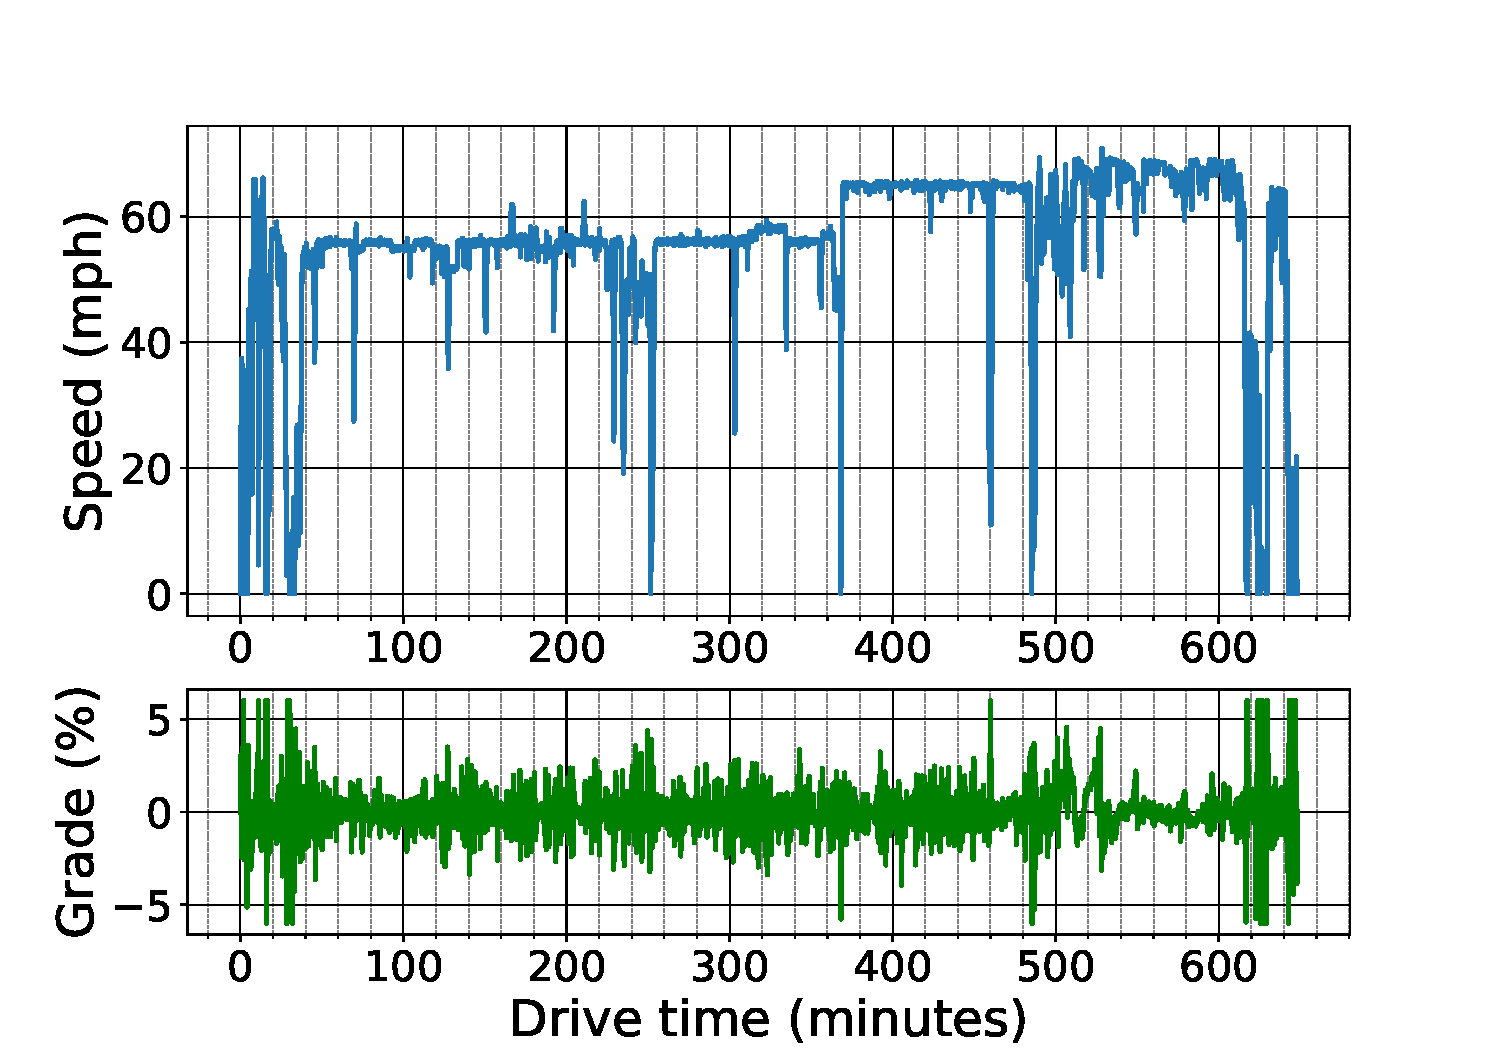
\includegraphics[width=\textwidth]{figures/long_haul_drivecycle.pdf}
        \caption{Drivecycle used for the long-haul truck simulation in \cite{Sader_2023}.}
        \label{fig:long_haul_drivecycle}
    \end{subfigure}
    \hfill
    \begin{subfigure}[b]{0.49\textwidth}
        \centering
        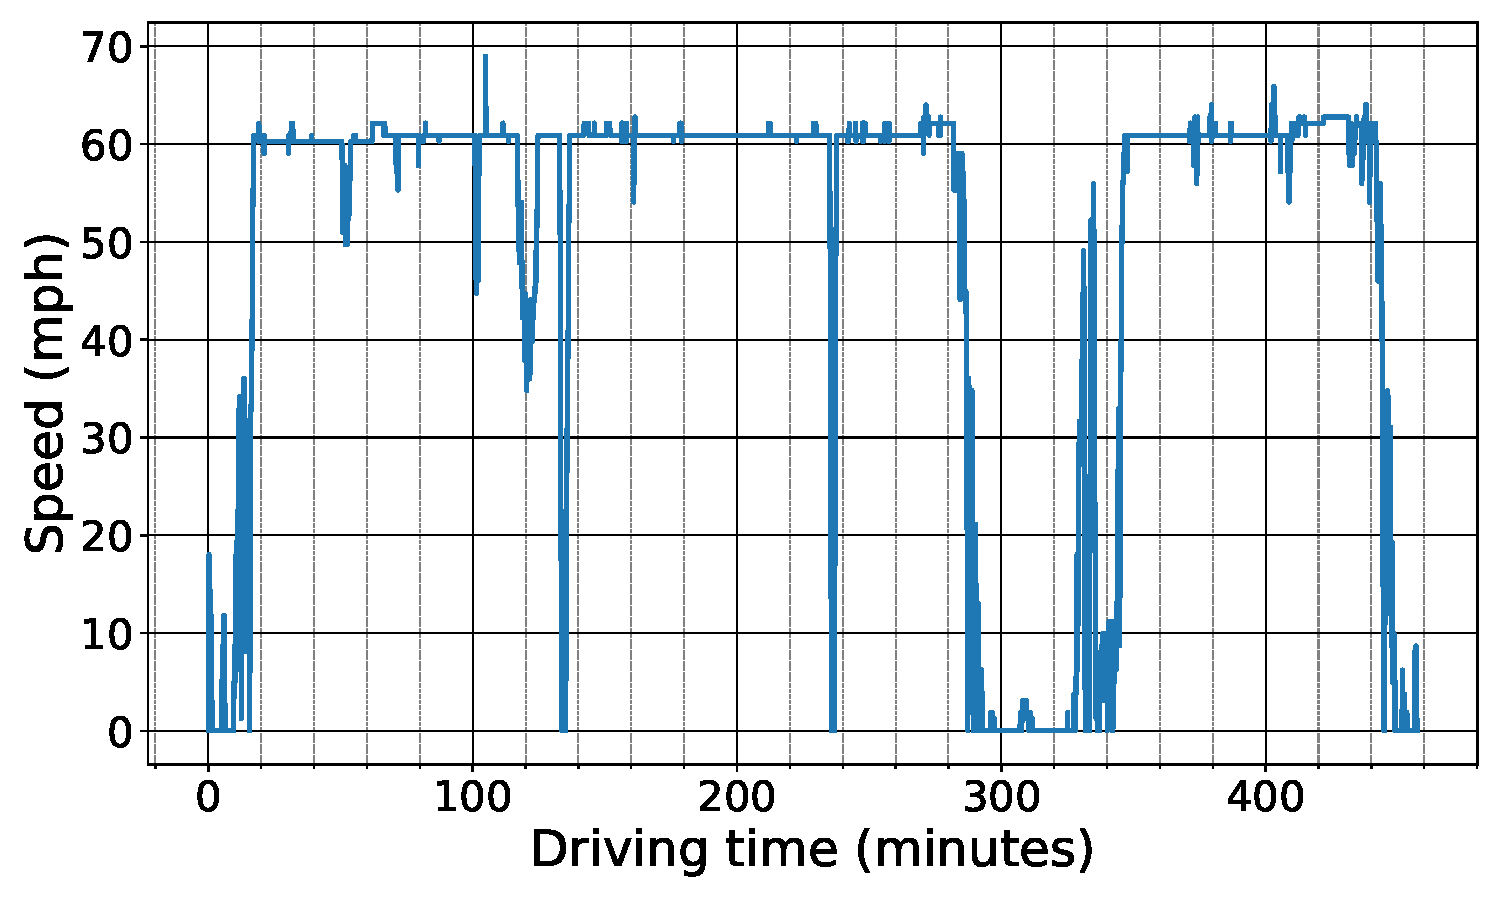
\includegraphics[width=\textwidth]{figures/pepsi_3_drive_cycle_24_paper.pdf}
        \caption{Sample drivecycle from PepsiCo's Tesla Semi pilot}
        \label{fig:sample_pepsico_drivecycle}
    \end{subfigure}
    \caption{Comparison of long-haul drivecycle used in Ref. \cite{Sader_2023} with a sample drivecycle from PepsiCo's 2023 Tesla Semi pilot}
    \label{fig:drivecycles}
\end{figure}

Starting from the \href{https://colab.research.google.com/drive/124rFu_4vHx4cP6SODtdzCxnUmLY50wbW?usp=sharing}{open-source google colab notebook} published as supplementary material with Ref. \cite{Sader_2023}, the model was adapted to represent the Tesla Semi, based on performance data published from three Semis used in a 2023 pilot carried out by PepsiCo in partnership with the \textit{Run on Less - Electric DEPOT demonstration} \cite{NACFE_2023}. Figure \ref{fig:sample_pepsico_drivecycle} shows a sample drivecycle from this pilot, which excludes road grade information because this data was not collected during the NACFE pilot. 

\subsubsection{Impact of Neglecting Road Grade}

The truck simulation model presented in Ref. \cite{Sader_2023} accounts for the impact of road grade on the instantaneous power demand to the truck battery. However, the drivecycle datasets from PepsiCo's Tesla Semi pilot with NACFE do not include road grade information. Therefore, prior to adapting the model using these drivecycle datasets, we quantified the impact of neglecting the road grade information in the long-haul drivecycle shown in Figure \ref{fig:long_haul_drivecycle} on the cost and emission results of the original model. 

As shown in Figure \ref{fig:road_grade_comparison}, neglecting road grade induces a 1-3\% underestimate of different components of the total cost of truck ownership, and a 2.85-2.95\% underestimate of well-to-wheel emissions. These systematic effects are well within the uncertainties of other components of the cost and emissions calculations, such as the capital and electricity costs and grid emission intensity, and are thus considered negligible. 

\begin{figure}[H]
    \centering
    \begin{subfigure}[b]{0.55\textwidth}
        \centering
        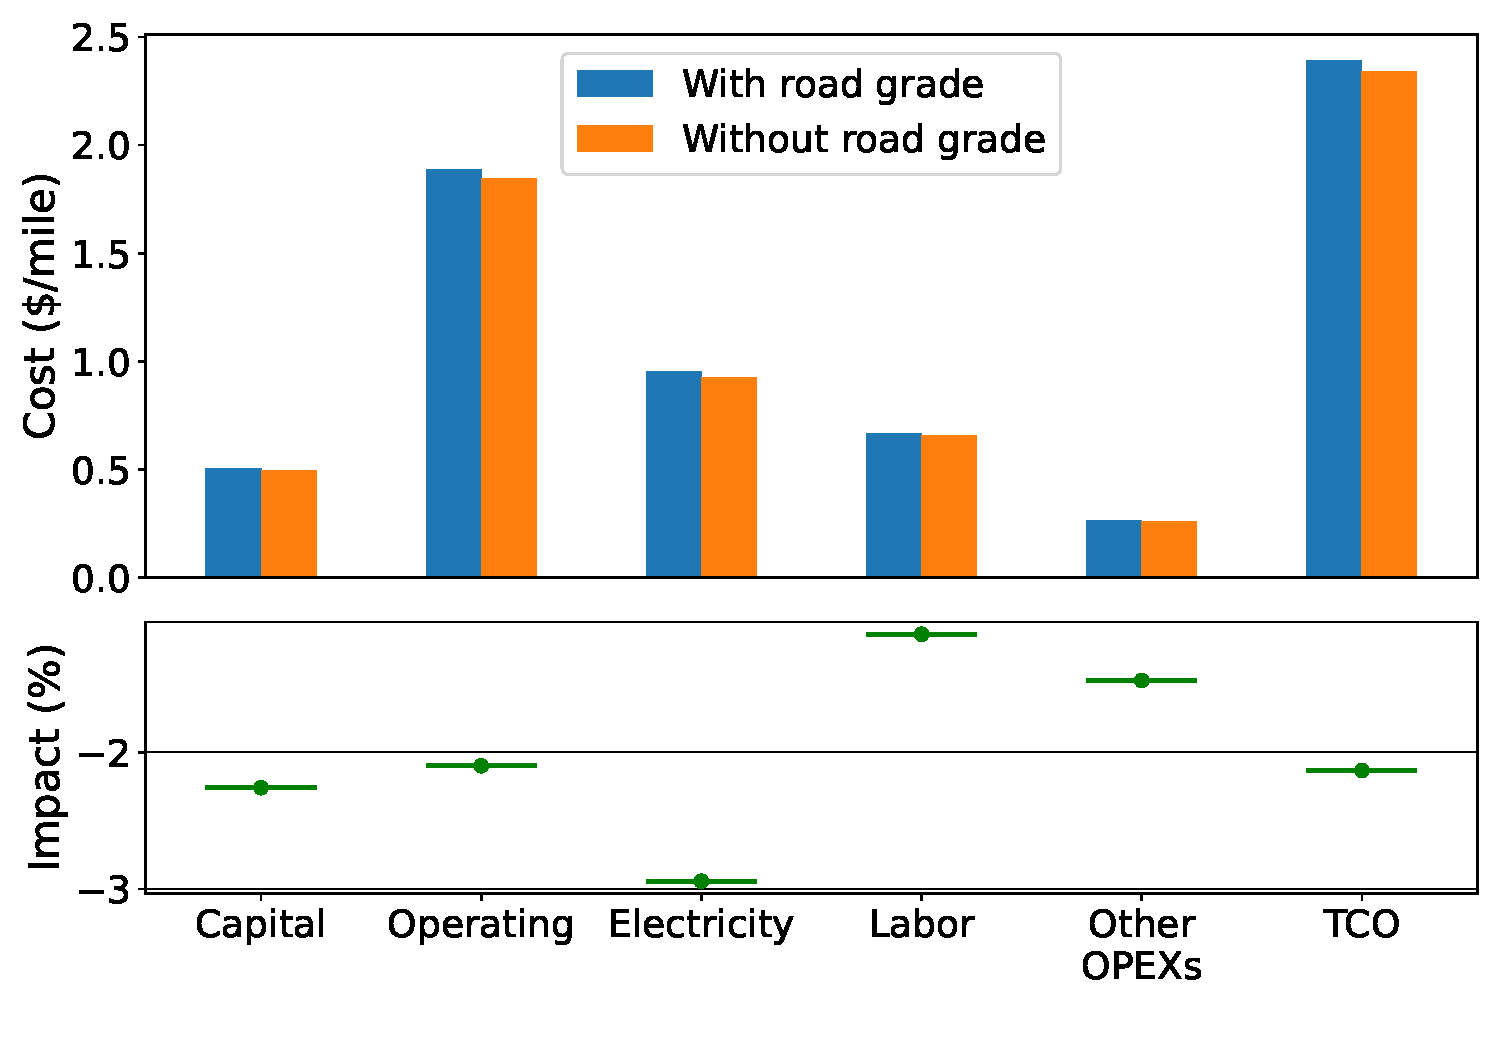
\includegraphics[width=\textwidth]{figures/results_comparison_costing.pdf}
        \caption{Total cost of ownership}
        \label{fig:results_comparison_costing}
    \end{subfigure}
    \hfill
    \begin{subfigure}[b]{0.43\textwidth}
        \centering
        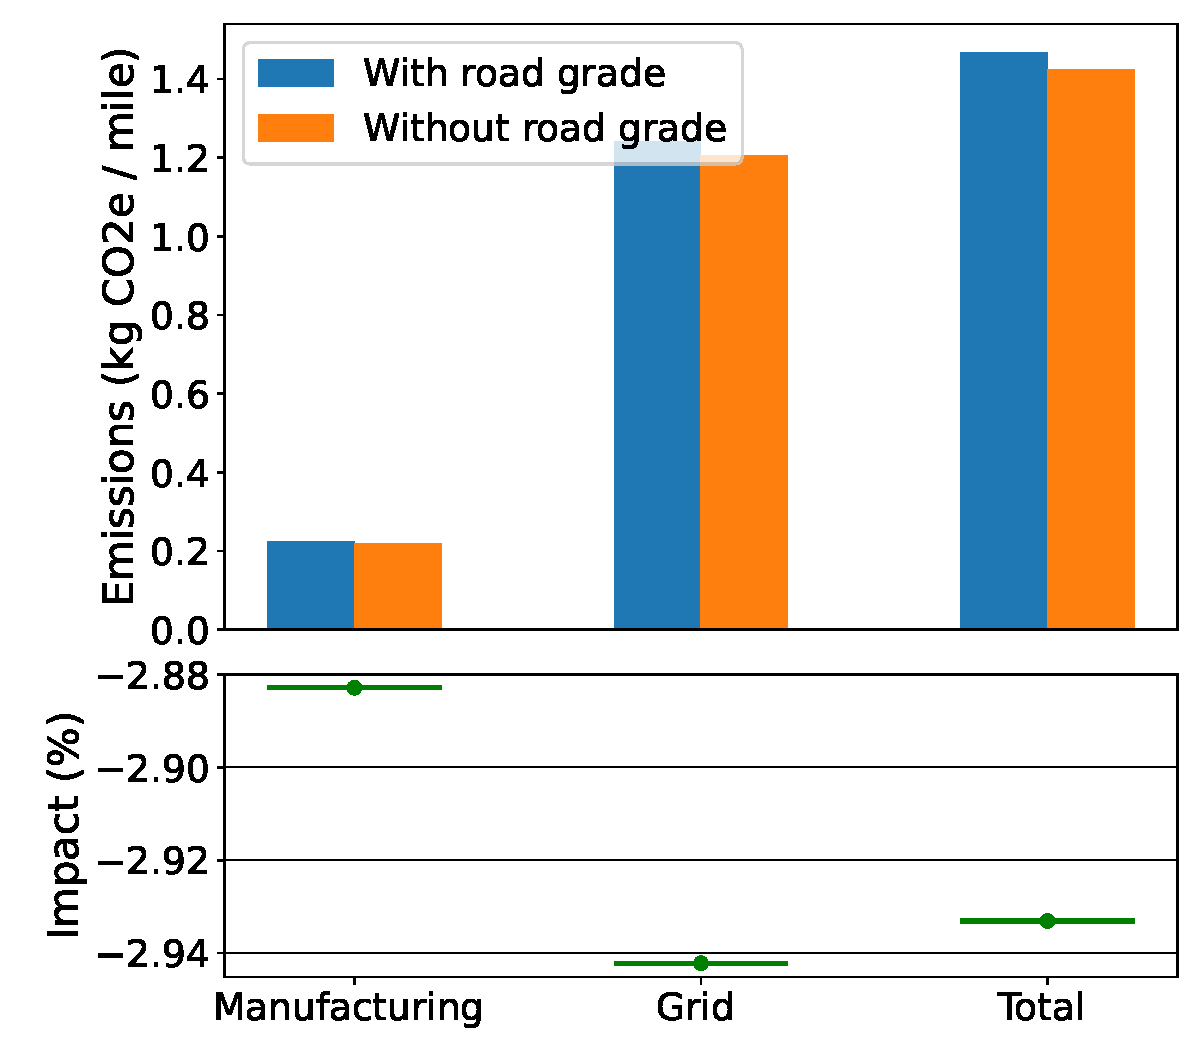
\includegraphics[width=\textwidth]{figures/results_comparison_emissions.pdf}
        \caption{Well-to-wheel emissions}
        \label{fig:results_comparison_emissions}
    \end{subfigure}
    \caption{Impact of neglecting road grade on major components of total cost of ownership (left) and well-to-wheel emissions (right) calculations using the model presented in Sader et al. \cite{Sader_2023}}
    \label{fig:road_grade_comparison}
\end{figure}

\subsubsection{Analysis of Tesla Semi Performance Data}
\label{sec:semi_performance_data}

\subsubsubsection{Drivecycle Extraction}

Twenty drivecycles are extracted from second-by-second performance data collected by onboard Geotab GO9 devices \cite{Geotab_2024} installed on the three trucks involved in PepsiCo's 2023 Tesla Semi pilot \cite{NACFE_2023}. Table \ref{tab:nacfe_performance_data} summarizes the performance data information used in this analysis. An individual drivecycle is defined as a period between charging events during which the battery is registered as either losing energy to driving or gaining it to regenerative braking. The green bands in Figure \ref{fig:pepsi_3_drivecycles} represent individual drivecycles identified in the data collected from one of the three trucks. 

\begin{table}[H]
\centering
\begin{tabular}{P{4cm}P{10cm}} % Adjust the column widths as needed
\toprule % Thicker top line
\textbf{Information} & \textbf{Description} \\ \midrule % Midrule for under header
Timestamp & Timestamp, down to 1-second precision. Adjacent timestamps are typically separated by 1 second, but longer breaks occur occasionally. \\
\midrule % Thin line between rows
Speed & Moving speed of the truck, in miles per hour (mph) \\
\midrule
Distance & Cumulative distance traveled (miles) \\
\midrule
State of Charge & Battery state of charge (\%) \\
\midrule
Energy Type & Mode in which the battery is accumulating or losing energy. Data from the Semis included following modes: \verb|driving_energy| (energy lost while driving), \verb|energy_regen| (energy gained from regenerative braking), and \verb|energy_from_dc_charger| (energy gained from DC charging). \\
\midrule
Accumulated Battery Energy & Battery energy accumulated (if Energy Type is \verb|energy_from_dc_charger| or \verb|energy_regen|) or lost (if Energy Type is \verb|driving_energy|) \\
\bottomrule % Thicker bottom line
\end{tabular}
\caption{Summary of information from Tesla Semi pilot performance data used in the analysis. The data was collected from three trucks operated by PepsiCo during the pilot, and published by NACFE as part of the \textit{Run on Less - Electric DEPOT demonstration} \cite{NACFE_2023}.}
\label{tab:nacfe_performance_data}
\end{table}

\begin{figure}[H]
        \centering
        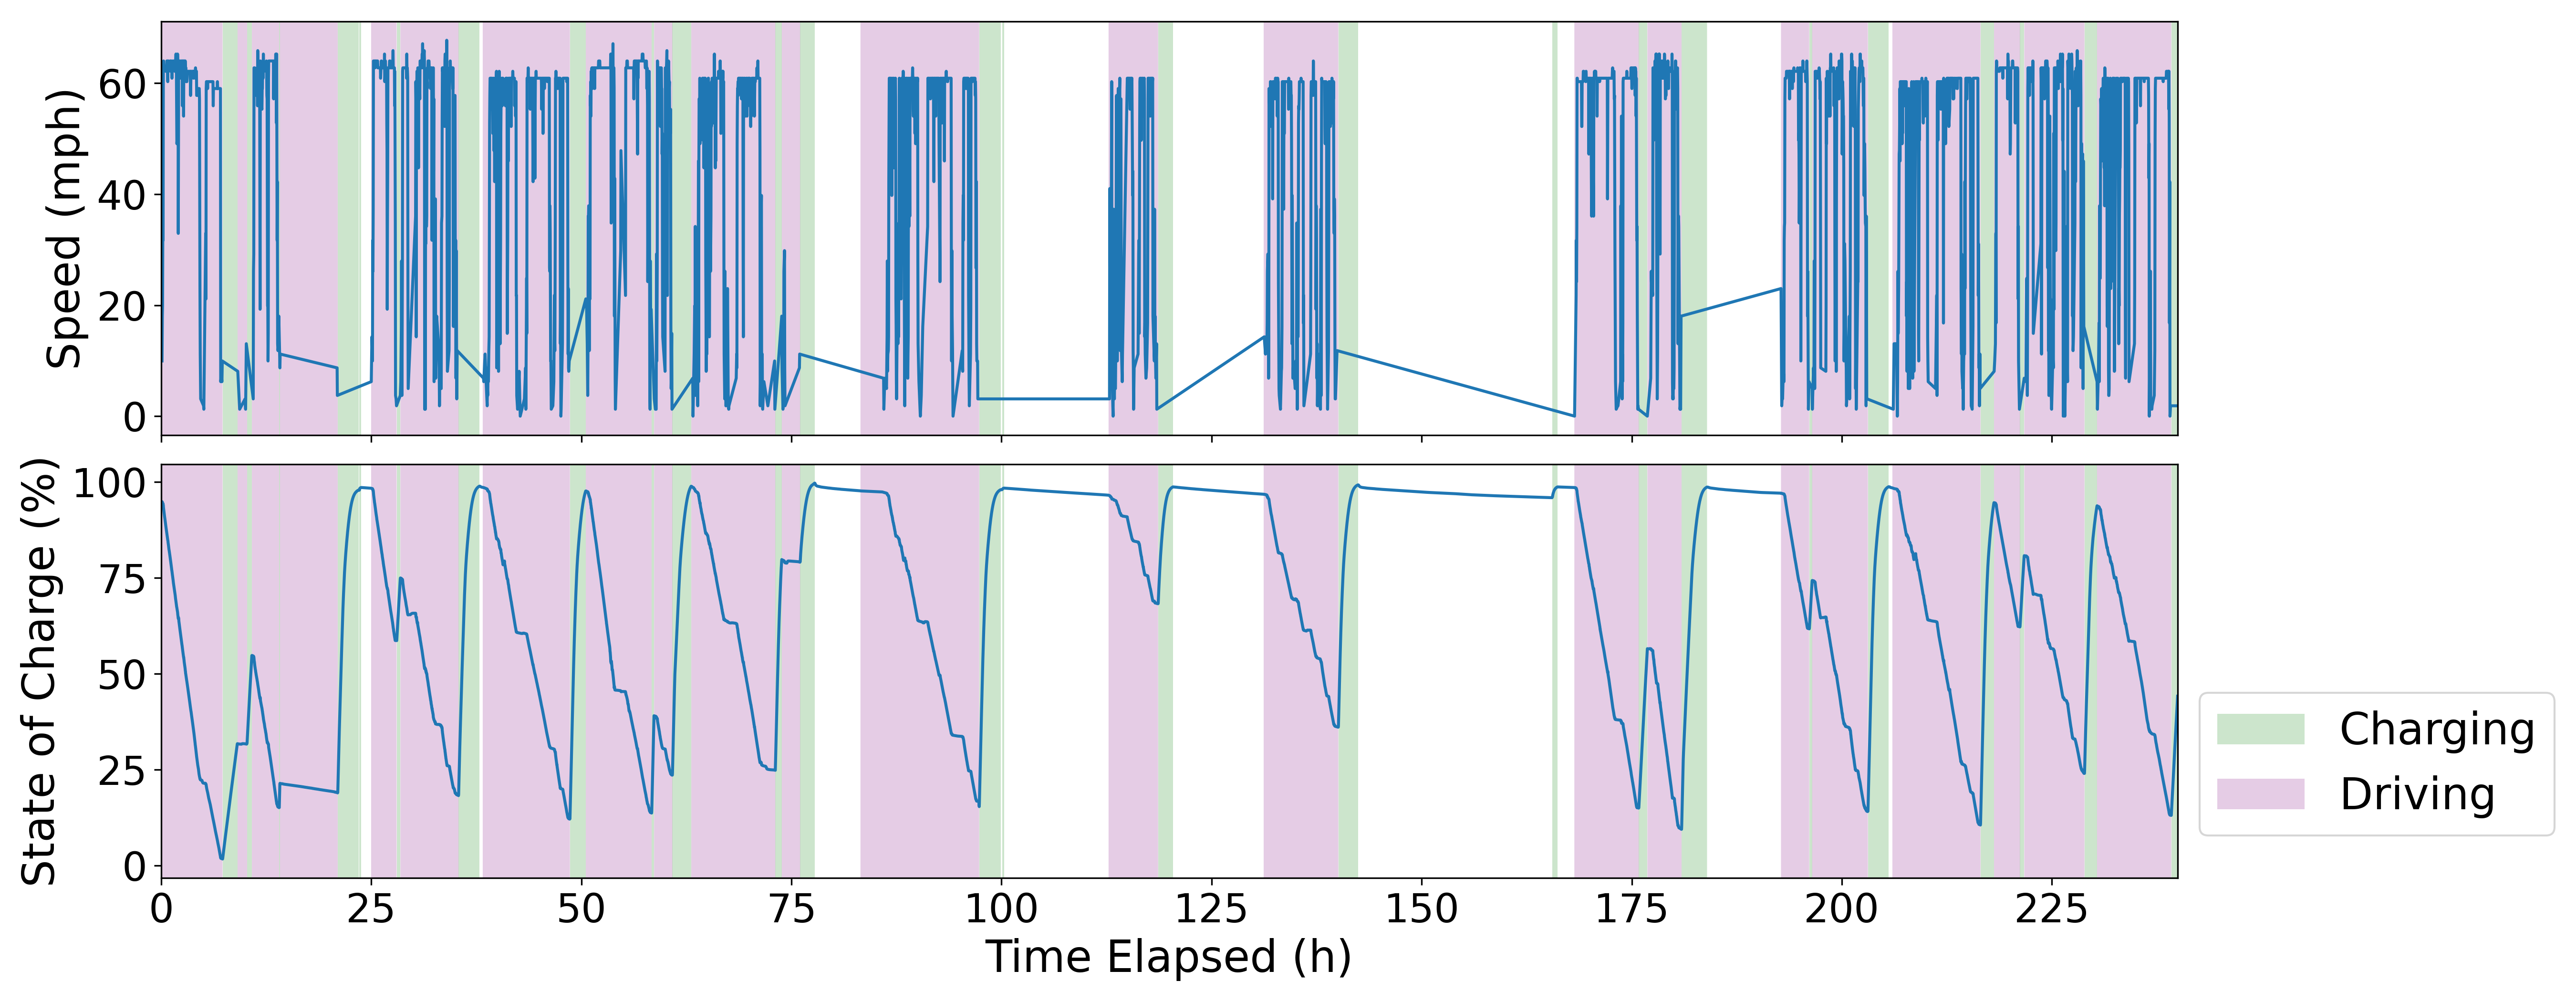
\includegraphics[width=\textwidth]{figures/pepsi_3_speed_vs_time.pdf}
        \caption{Driving and charging periods identified in the geotab data collected from the \textit{Pepsi 3} truck.}
        \label{fig:pepsi_3_drivecycles}
\end{figure}

\subsubsubsection{Evaluation of Battery Capacity}

The performance data is used to evaluate the battery capacity within each charging period, and the vehicle range and energy economy within each drivecycle.

Within a given charging period, the battery capacity is evaluated by fitting a quadratic function to the accumulated battery energy as a function of the reported state of charge using least squares regression, and extrapolating to the full charge range.

In principle, the battery energy would be expected to increase linearly with the state of charge, but in practice a quadratic fit is generally seen to yield significant improvement relative to linear, as measured by root mean squared error (RMSE). This is illustrated for a sample charging event in Figure \ref{fig:charging_fits}.

\begin{figure}[H]
    \centering
    \begin{subfigure}[b]{0.48\textwidth}
        \centering
        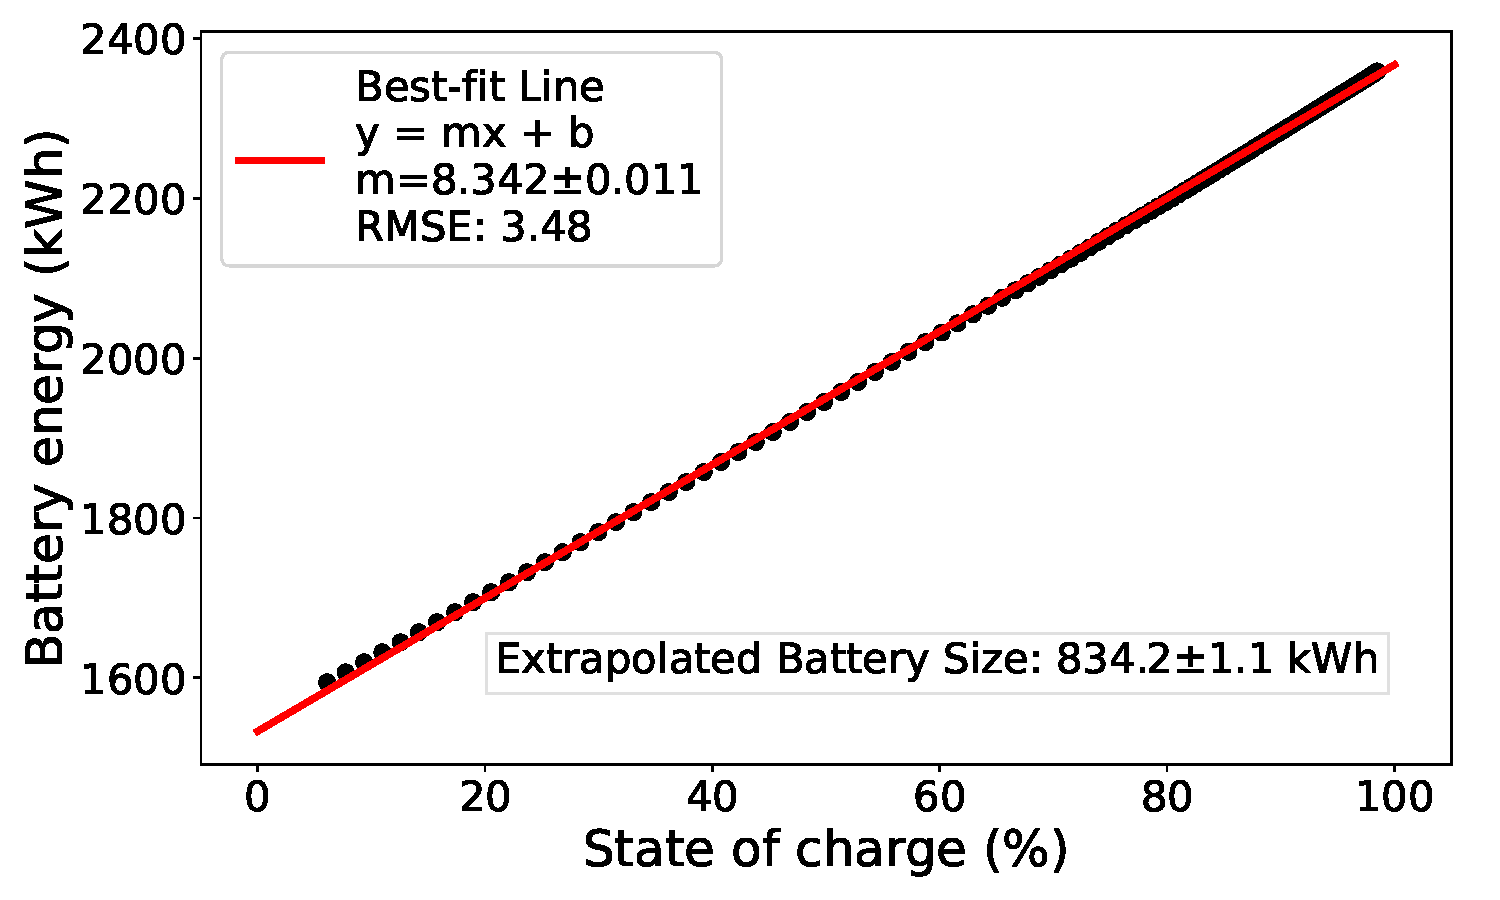
\includegraphics[width=\textwidth]{figures/pepsi_1_battery_soc_vs_energy_event_11_linearfit.pdf}
        \caption{Linear fit}
        \label{fig:charging_linear_fit}
    \end{subfigure}
    \hfill
    \begin{subfigure}[b]{0.48\textwidth}
        \centering
        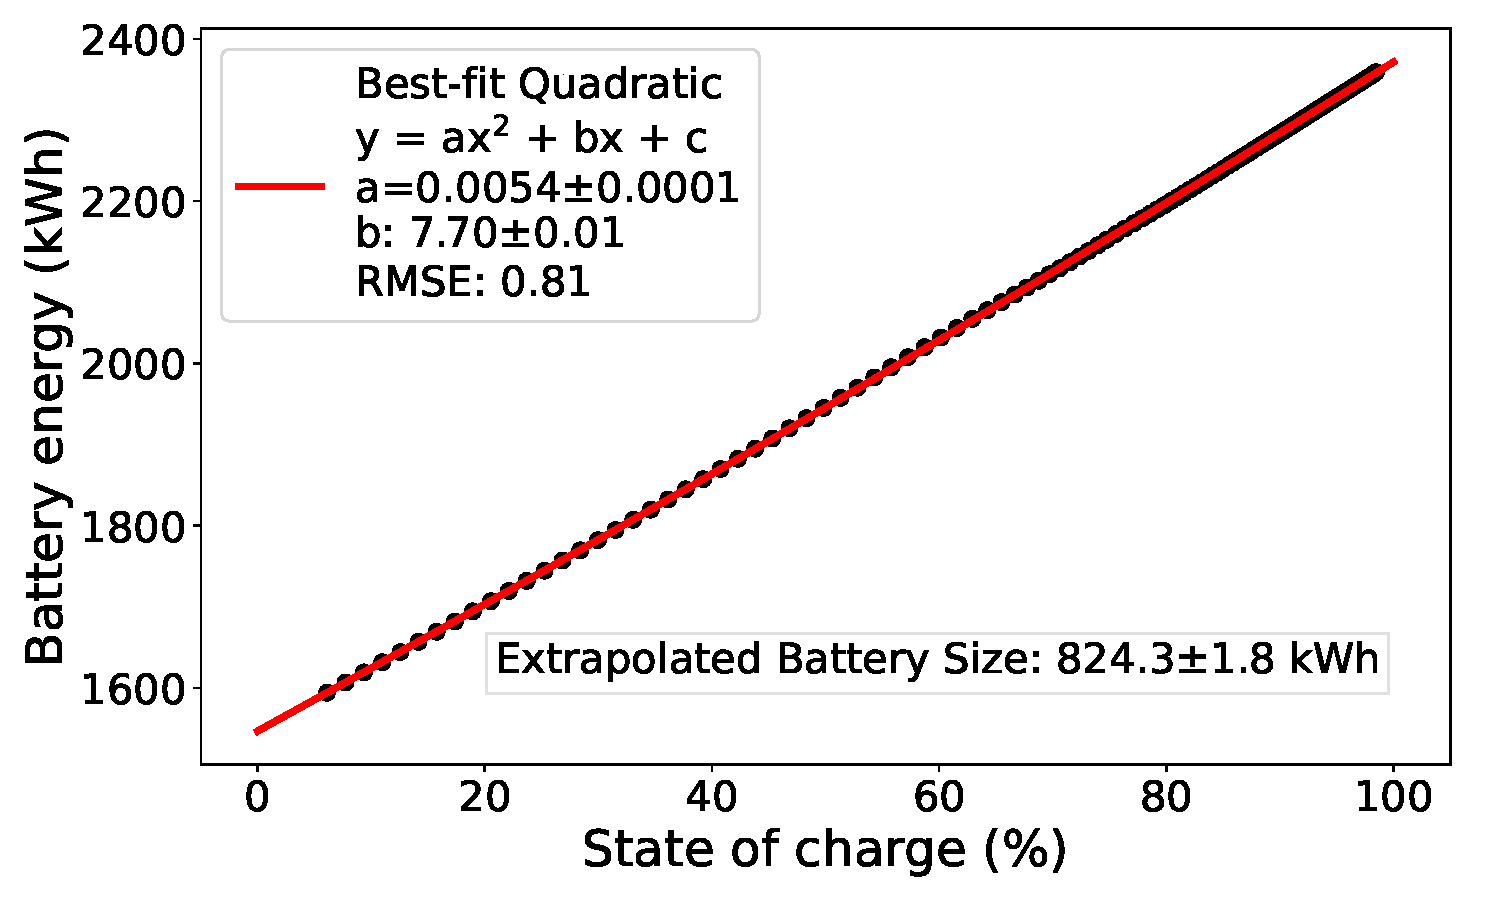
\includegraphics[width=\textwidth]{figures/pepsi_1_battery_soc_vs_energy_event_11_quadfit.pdf}
        \caption{Quadratic fit}
        \label{fig:charging_quad_fit}
    \end{subfigure}
    \caption{Comparison of linear and quadratic fits to the battery energy as a function of state of charge for a sample charging event collected from the \textit{Pepsi 1} truck.}
    \label{fig:charging_fits}
\end{figure}

For each fit, the battery size was extrapolated from the fitting function $f_\text{fit}$ as:

\begin{equation}
    \text{Battery size}_\text{charging event i} = f_\text{fit, i}(\text{State of charge = 100\%}) - f_\text{fit, i}(\text{State of charge = 0\%})
\end{equation}

For a given truck, the battery capacity is estimated using the weighted mean over all charging events that contain at least 10 data points and recharge at least 50\% of the battery's state of charge:

\begin{equation}
    \overline{\text{Battery size}}_\text{truck j} = \frac{\sum_\text{event i}^\text{N} (\text{Battery size}_i/\sigma_i)^2}{\sum_\text{event i}^\text{N}(1/\sigma_i)}
\end{equation}

where $N$ is the total number of charging events that pass the criteria for the given truck, and $\sigma_i$ is the uncertainty in the evaluated battery size for charging event $i$ in truck $j$. The uncertainty $\delta(\text{Battery size}_\text{truck j})$ is evaluated using the weighted standard deviation:

\begin{equation}
    \delta(\text{Battery size}_\text{truck j}) = \sqrt{\frac{\sum (\frac{1}{\sigma_i^2}) (\text{Battery size}_i - \overline{\text{Battery size}}_\text{truck j})^2}{\sum \frac{1}{\sigma_i}^2}}
\end{equation}

Figure \ref{fig:battery_capacity_summary} shows the extrapolated battery capacities for a sample truck and the weighted mean over all drivecycles. The results are summarized in Table \ref{tab:battery_capacity_summary}, with a weighted mean battery capacity of (823 $\pm$ 2) kWh over all three Semi trucks.

\begin{figure}[H]
        \centering
        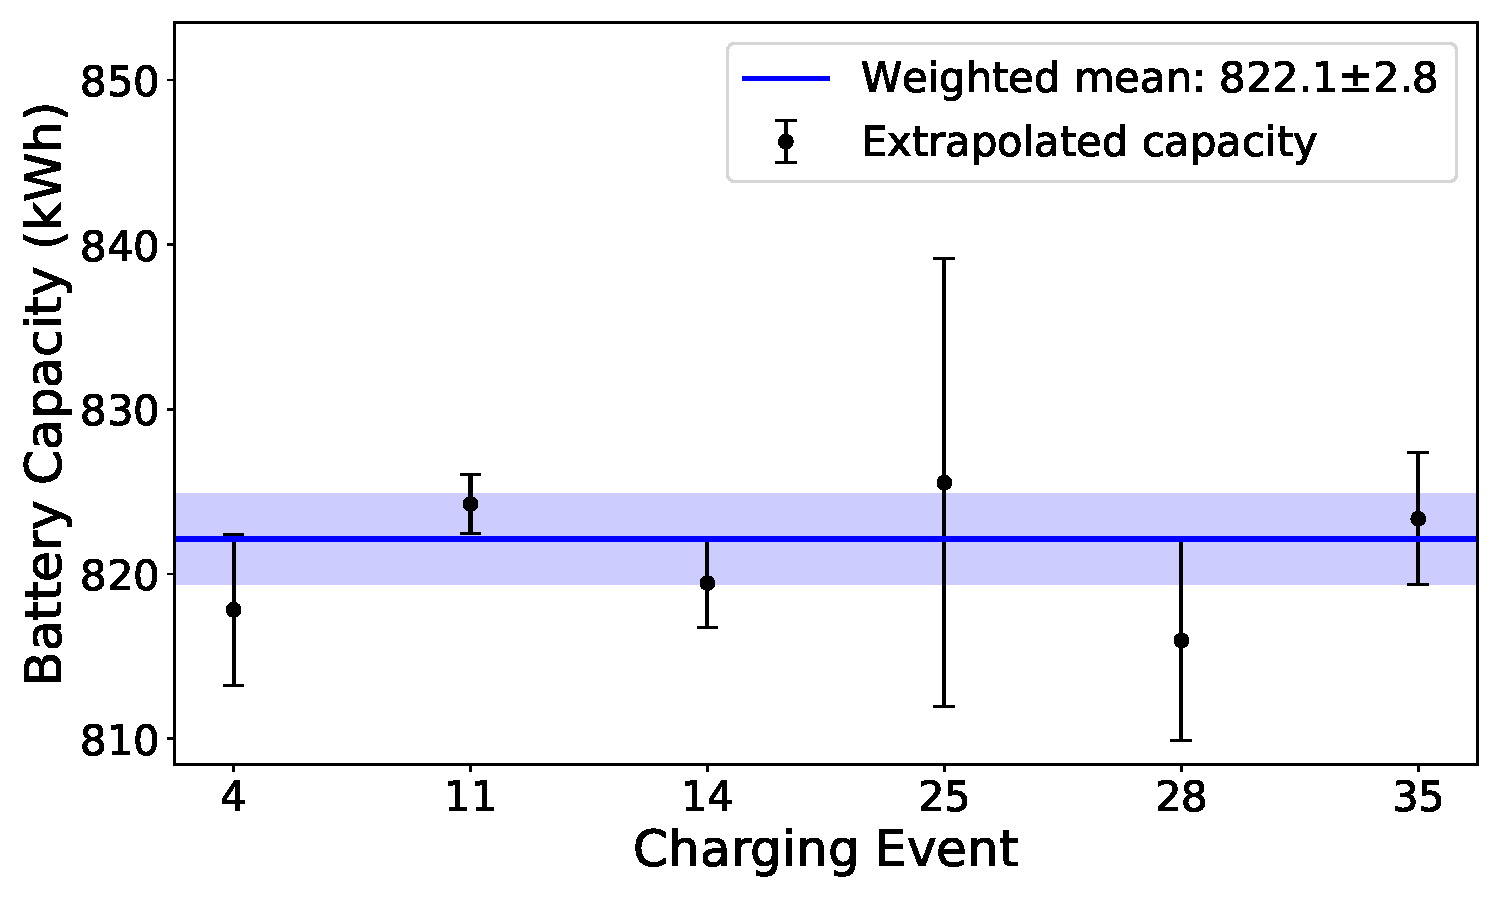
\includegraphics[width=0.6\textwidth]{figures/pepsi_1_battery_capacity_summary.pdf}
        \caption{Summary of battery capacity estimates extrapolated from quadratic fits to battery energy as a function of state of charge for the \textit{Pepsi 1} truck}
        \label{fig:battery_capacity_summary}
\end{figure}

\begin{table}[H]
\centering
\begin{tabular}{P{4cm}P{6cm}} % Adjust the column widths as needed
\toprule % Thicker top line
\textbf{Truck} & \textbf{Battery capacity (kWh)} \\ \midrule % Midrule for under header
Pepsi 1 & 822 $\pm$ 3 \\
\midrule
Pepsi 2 & 825 $\pm$ 7 \\
\midrule
Pepsi 3 & 827 $\pm$ 6 \\
\midrule
Combined & 825 $\pm$ 2 \\
\bottomrule % Thicker bottom line
\end{tabular}
\caption{Summary of battery capacity estimates for each Tesla Semi in the pilot, obtained using weighted mean over all analyzed charging events}
\label{tab:battery_capacity_summary}
\end{table}

\subsubsubsection{Evaluation of Truck Range and Energy Economy}

Within a given drivecycle, the range is extrapolated from a linear fit to the distance traveled as a function of state of charge, using a procedure analogous to that presented above to evaluate battery sizes. The energy economy for a given drivecycle is evaluated as:

\begin{equation}
    \text{Energy Economy}_\text{drivecycle i, truck j} = \frac{\text{DoD}_i * \text{Battery size}_\text{truck j}}{\text{Distance Traveled}_i}
\end{equation}

where the depth of discharge DoD is the relative loss of battery charge over the full drivecycle: $\text{DoD} = ((\text{state of charge})_\text{init} - \text{state of charge})_\text{final}) / 100\%$.

The distance vs. charge curves are generally found to fall into two classes, extreme examples of which are shown in Figure \ref{fig:distance_vs_soc}. The first class (``linear") is well-represented by a linear fit, whereas the second class (``non-linear") exhibits strong non-linearities. 

\begin{figure}[H]
    \centering
    \begin{subfigure}[b]{0.48\textwidth}
        \centering
        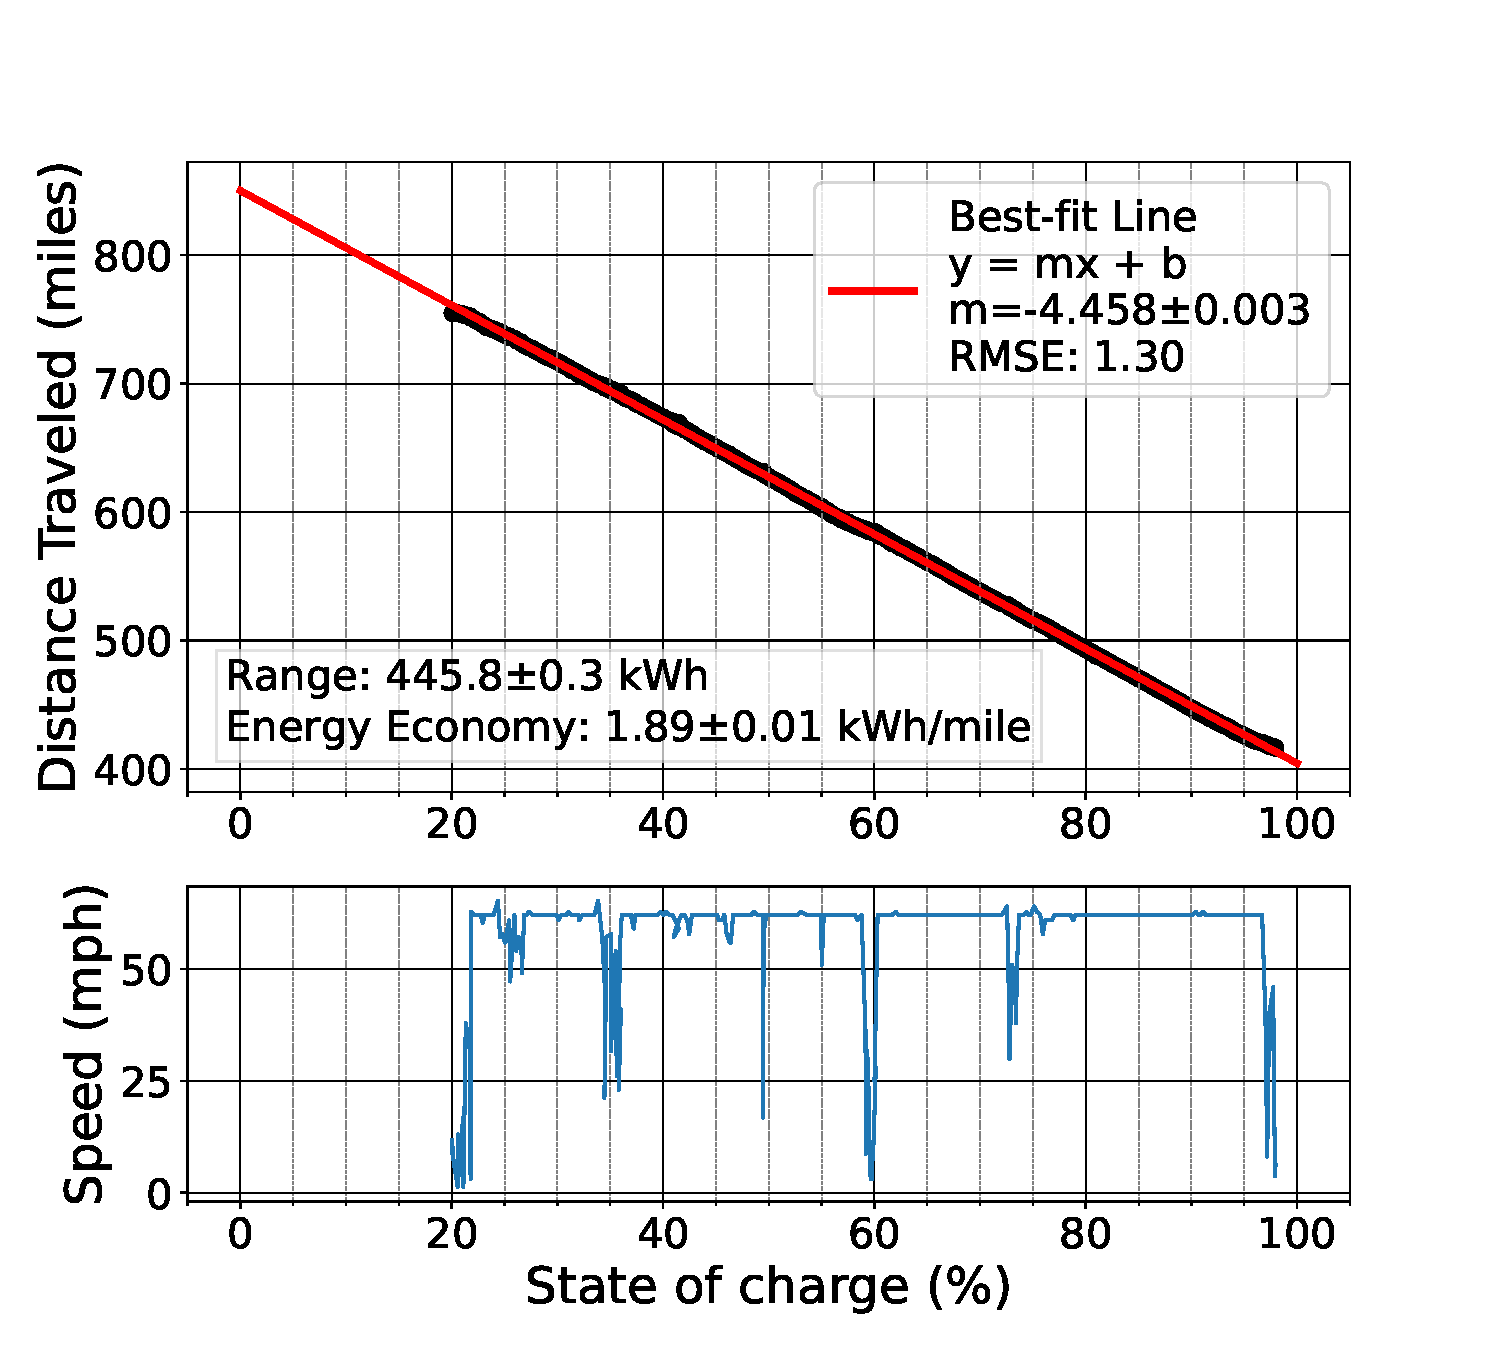
\includegraphics[width=\textwidth]{figures/pepsi_1_battery_soc_vs_distance_event_9_linearfit.pdf}
        \caption{Linear drivecycle}
        \label{fig:distance_vs_soc_linear}
    \end{subfigure}
    \hfill
    \begin{subfigure}[b]{0.48\textwidth}
        \centering
        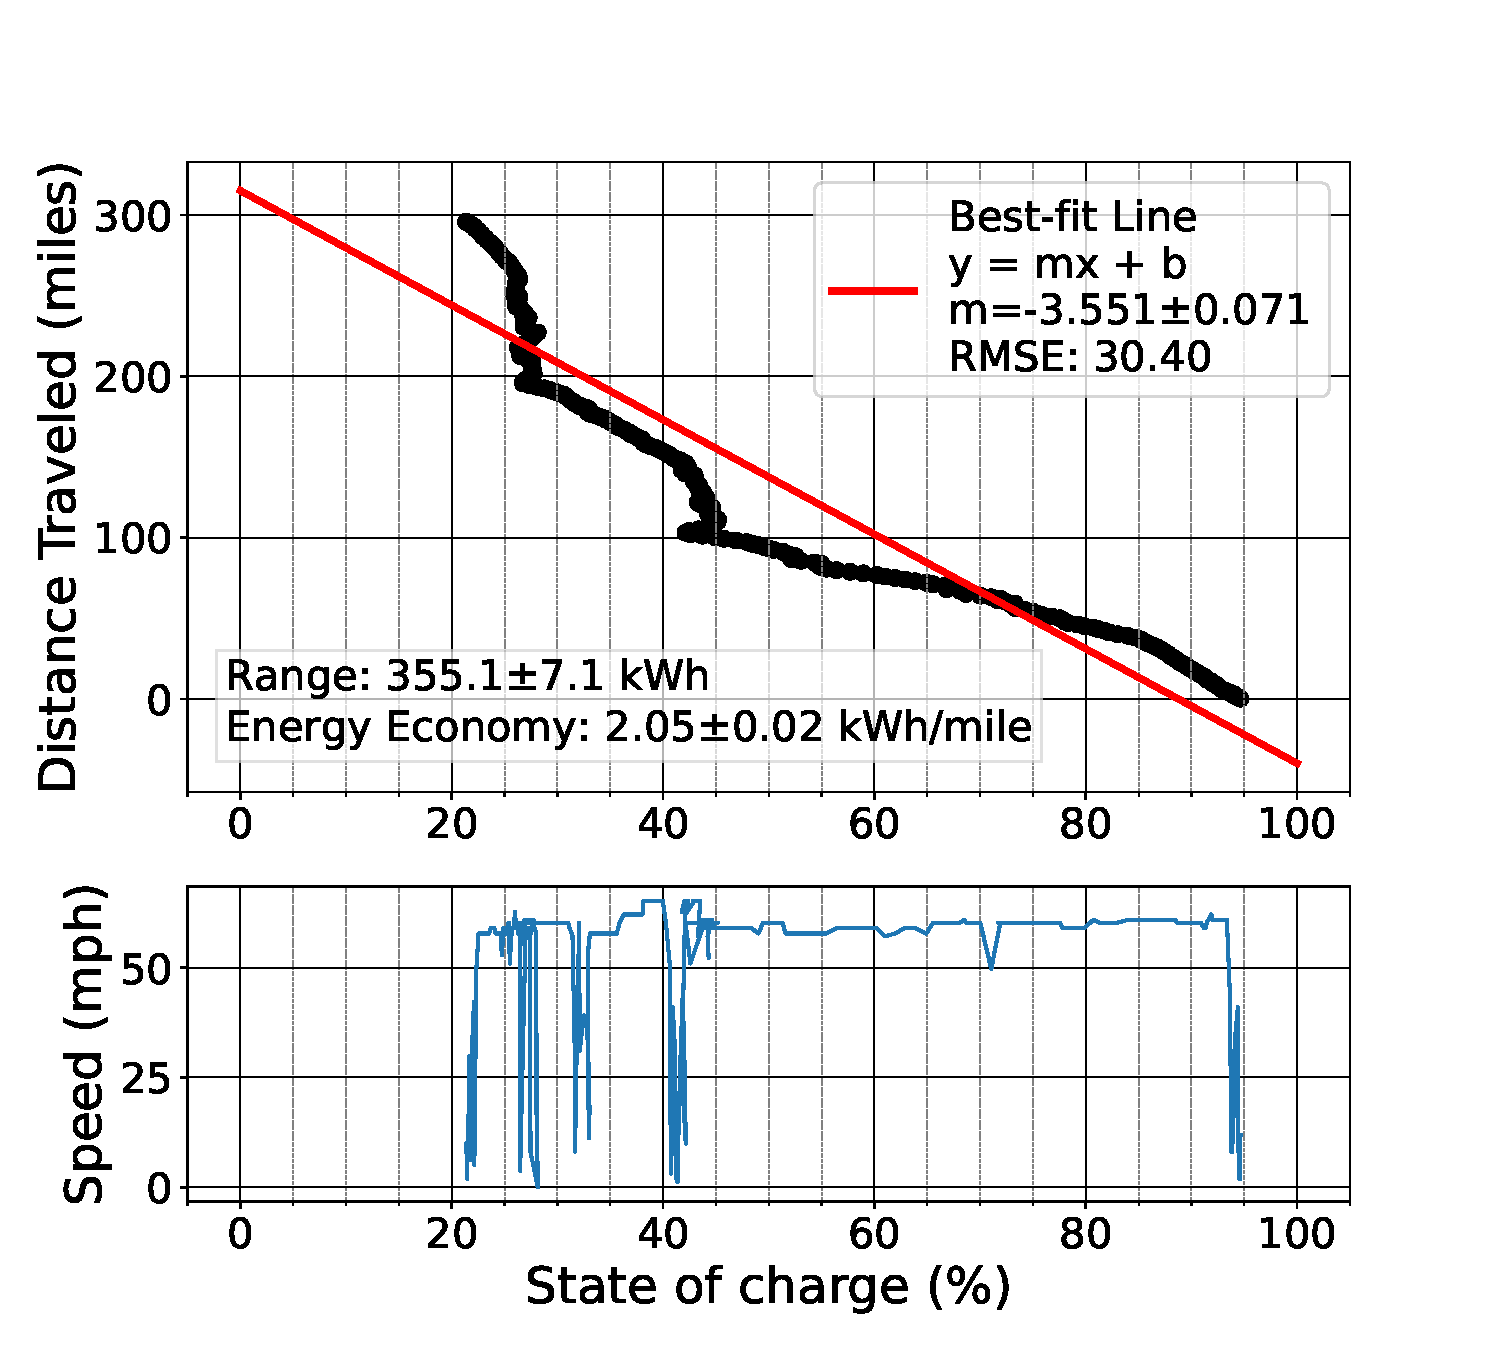
\includegraphics[width=\textwidth]{figures/pepsi_2_battery_soc_vs_distance_event_2_linearfit.pdf}
        \caption{Nonlinear drivecycle}
        \label{fig:distance_vs_soc_nonlinear}
    \end{subfigure}
    \caption{Sample drivecycles showing speed and distance traveled as a function of state of charge. The left-hand drivecycle is classified as ``linear", and the right-hand as ``nonlinear" on the basis of their linear fit RMSE.}
    \label{fig:distance_vs_soc}
\end{figure}

It's assumed that the non-linear curves represent roundtrips from Sacramento, CA to Reno, NV discussed in Ref. \cite{NACFE_2023}, which cover mountainous terrain that would be expected to incur significant variations on power demand to the battery, including regenerative braking on downhill sections. Conversely, the curves with strong linearity are assumed to represent operations in the vicinity of Sacramento, within the flat Central Valley region of California. 

The drivecycles are classified as linear or non-linear according to the RMSE of their linear fit. Figure \ref{fig:rmse_dist} shows the distribution of RMSE for linear fits over all drivecycles. An RMSE cutoff of 10 is placed to mark the boundary above which significant nonlinear behavior is observed. Figure \ref{fig:distance_vs_soc_cutoff} shows two sample drivecycles with RMSE near this cutoff. Figure \ref{fig:range_energy_economy_summary} shows the extrapolated ranges and energy economies for a sample truck, for drivecycles classified as linear vs. non-linear. The results are summarized for each truck in Table \ref{tab:range_energy_summary}. 

\begin{figure}[H]
        \centering
        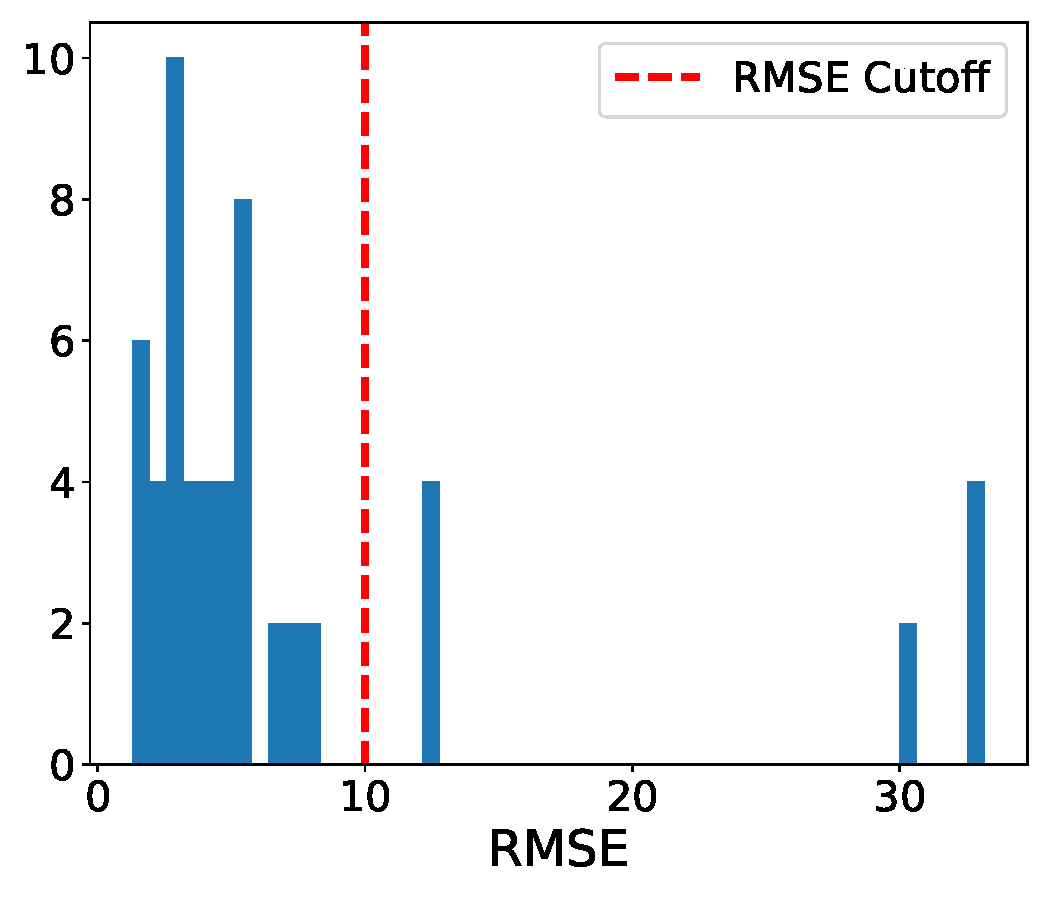
\includegraphics[width=0.5\textwidth]{figures/all_RMSE.pdf}
        \caption{Distribution of RMSE for linear fits to the distance traveled as a function of battery state of charge over all drivecycles. The red dashed line shows the placement of the RMSE cutoff for the ``linear" classification.}
        \label{fig:rmse_dist}
\end{figure}

\begin{figure}[H]
    \centering
    \begin{subfigure}[b]{0.48\textwidth}
        \centering
        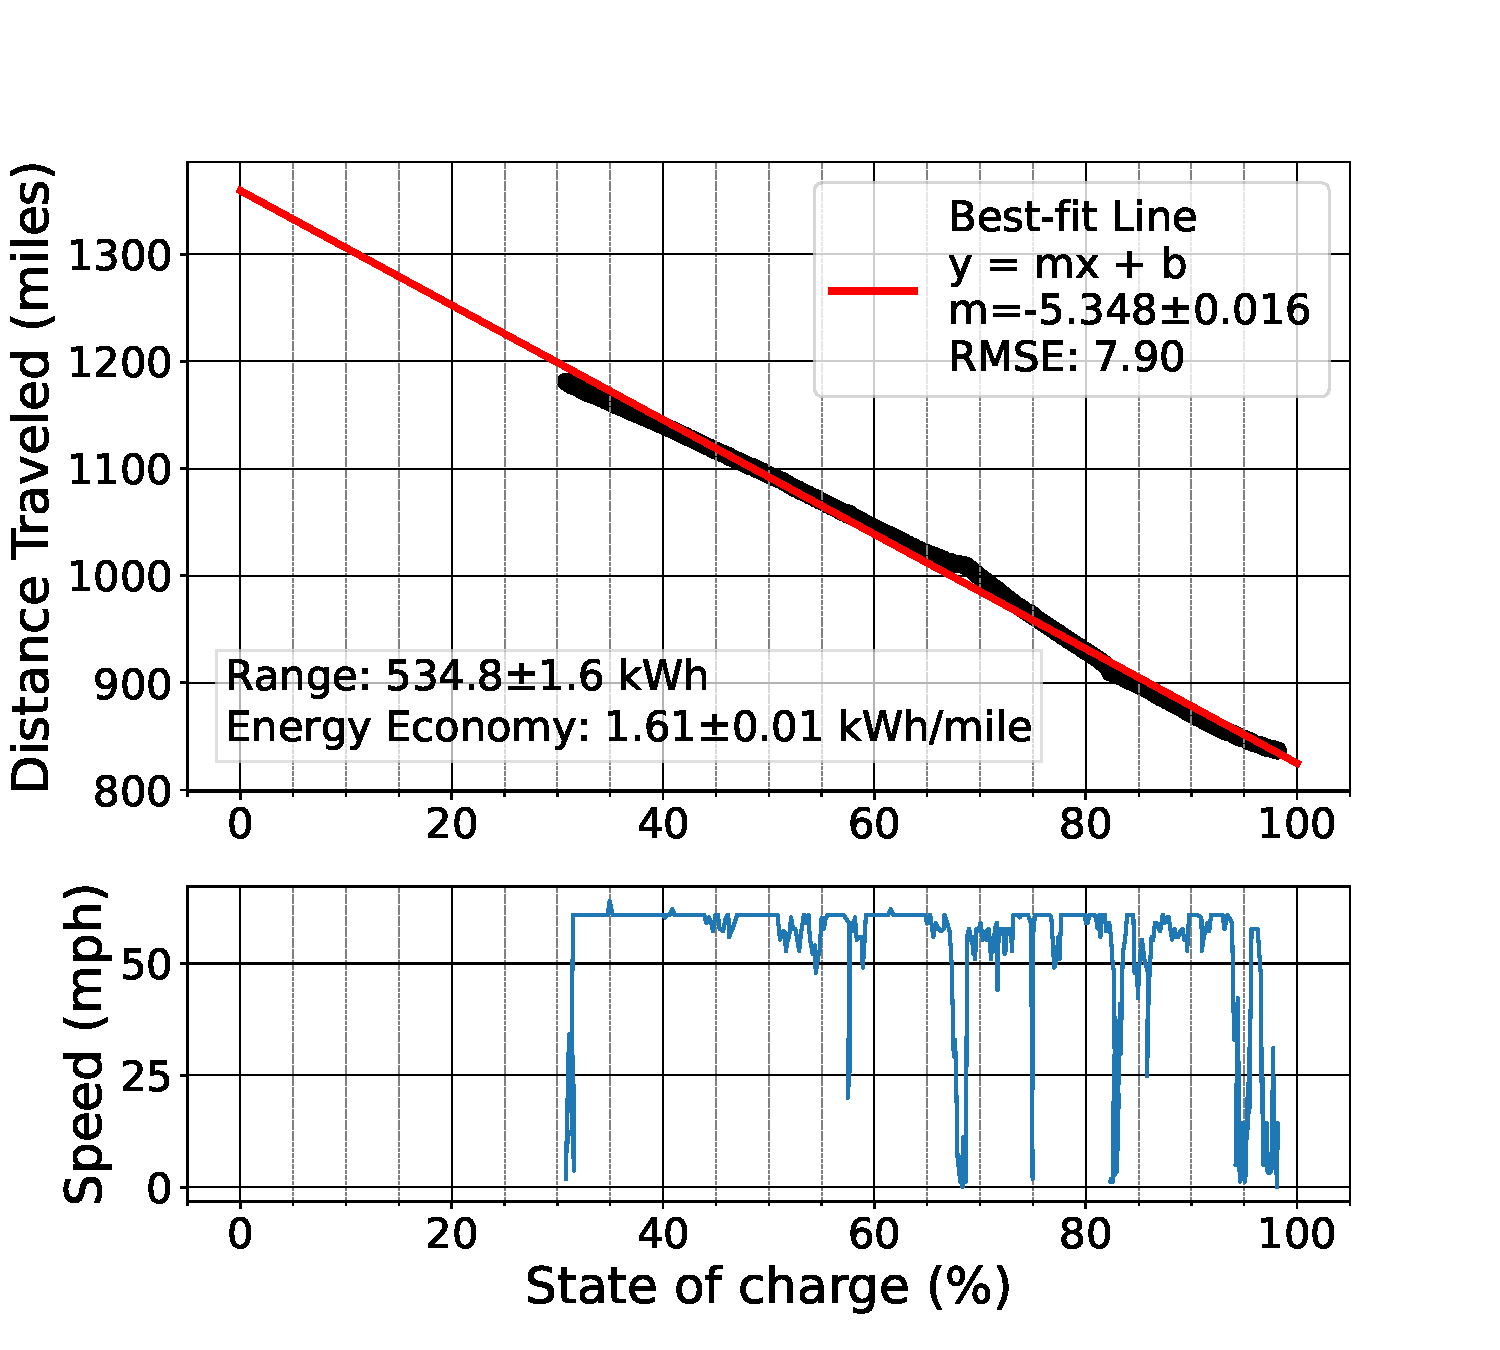
\includegraphics[width=\textwidth]{figures/pepsi_1_battery_soc_vs_distance_event_13_linearfit.pdf}
        \caption{RMSE = 7.90 (linear)}
        \label{fig:distance_vs_soc_below_cutoff}
    \end{subfigure}
    \hfill
    \begin{subfigure}[b]{0.48\textwidth}
        \centering
        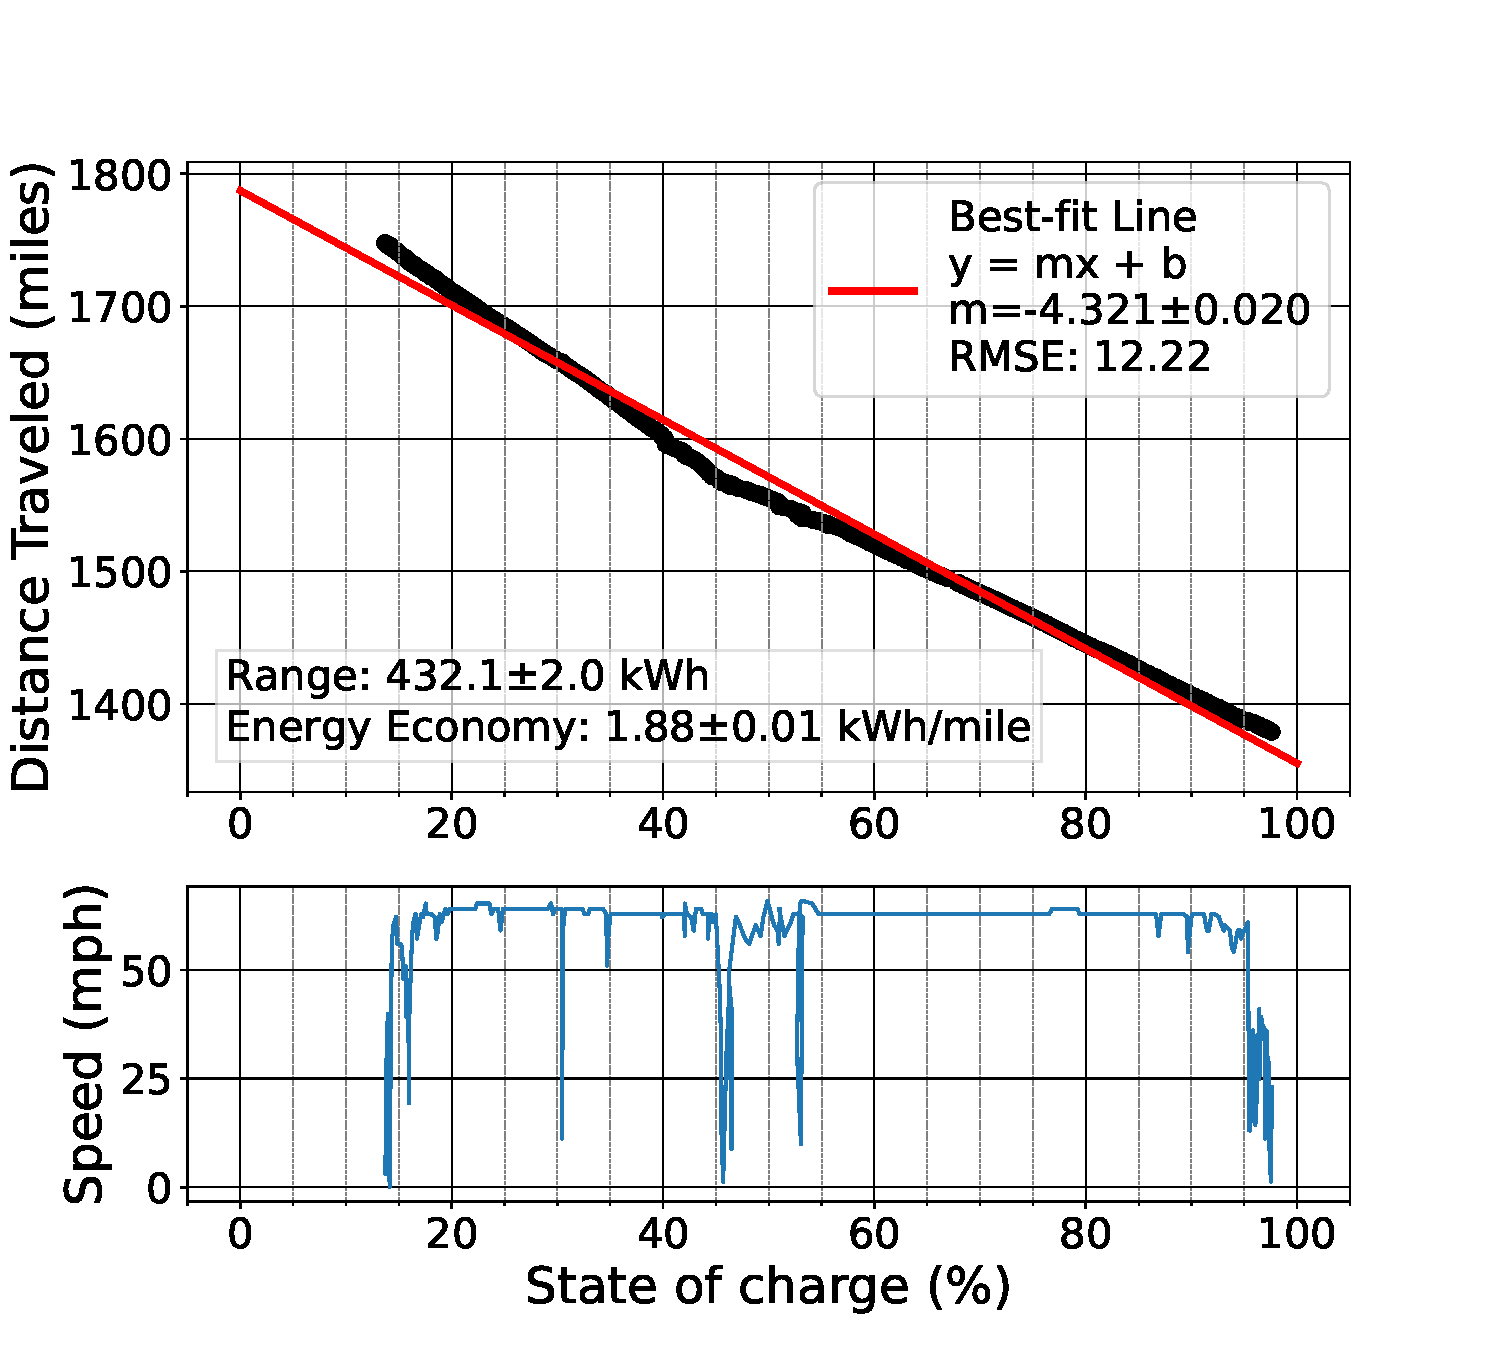
\includegraphics[width=\textwidth]{figures/pepsi_3_battery_soc_vs_distance_event_11_linearfit.pdf}
        \caption{RMSE = 12.22 (non-linear)}
        \label{fig:distance_vs_soc_above_cutoff}
    \end{subfigure}
    \caption{Sample drivecycles showing speed and distance traveled as a function of state of charge. The left-hand drivecycle has an RMSE falling just below the linearity cutoff of 5 (so is classified as ``linear), and the right-hand drivecycle falls just above the cutoff.}
    \label{fig:distance_vs_soc_cutoff}
\end{figure}

\begin{figure}[H]
    \centering
    \begin{subfigure}[b]{0.48\textwidth}
        \centering
        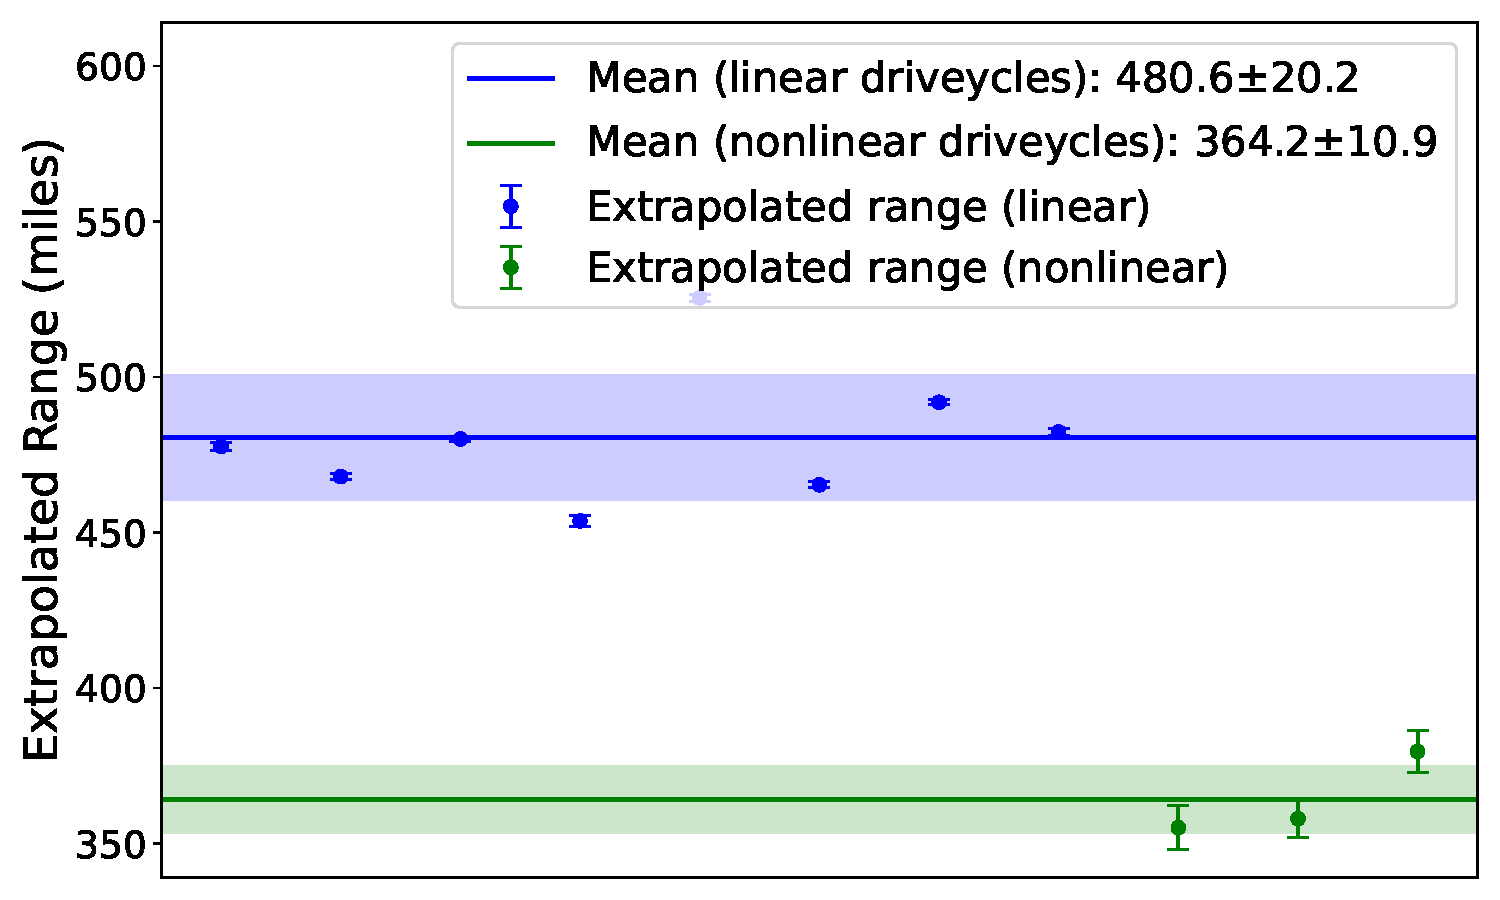
\includegraphics[width=\textwidth]{figures/pepsi_2_range_summary.pdf}
        \caption{Range estimates}
        \label{fig:range_summary}
    \end{subfigure}
    \hfill
    \begin{subfigure}[b]{0.48\textwidth}
        \centering
        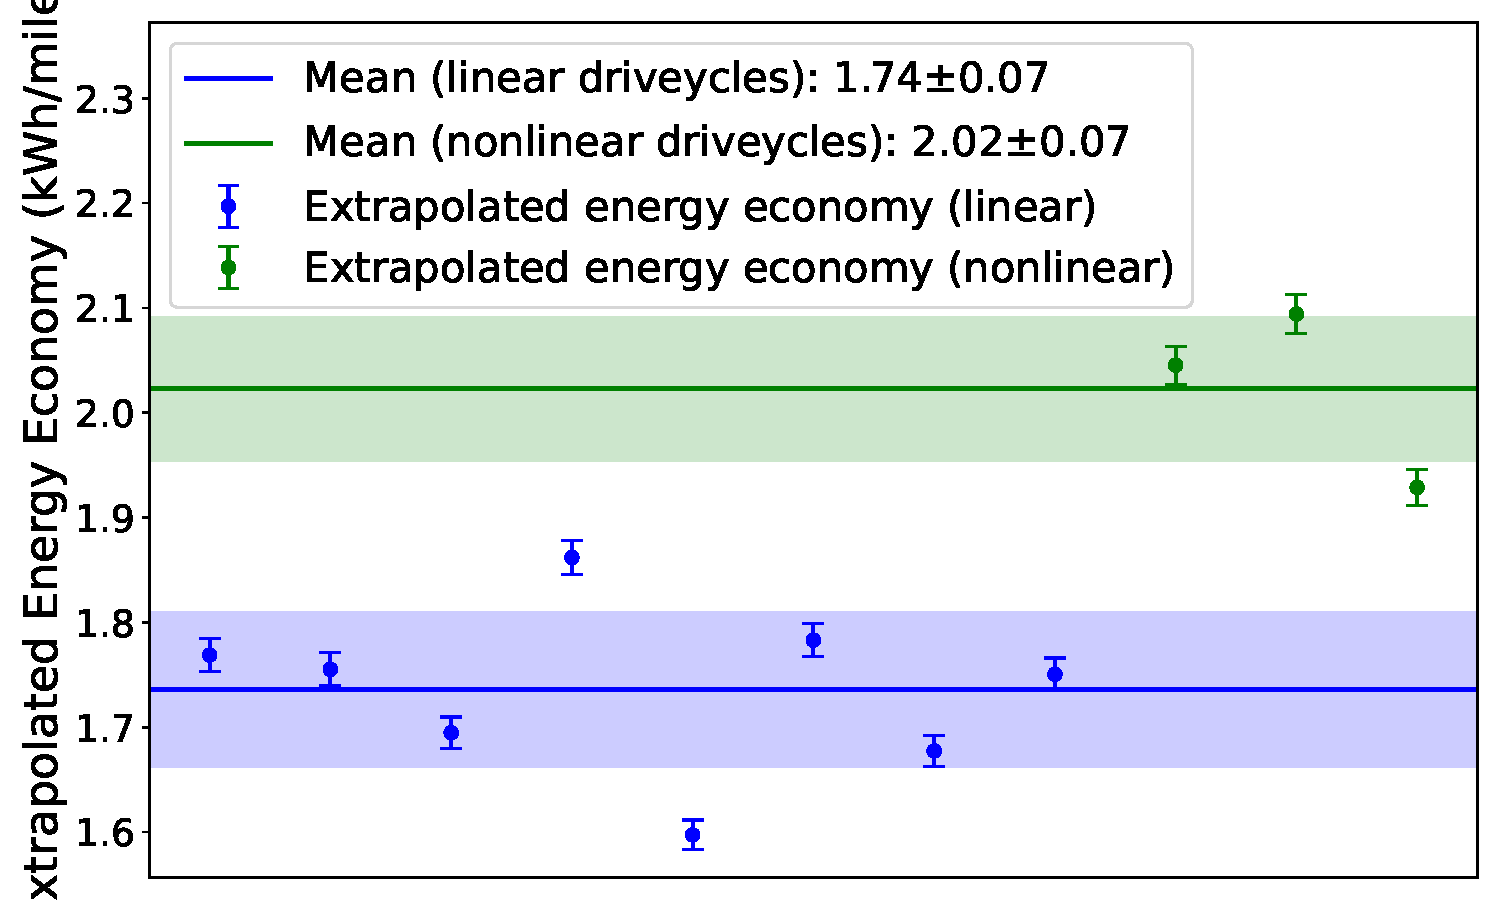
\includegraphics[width=\textwidth]{figures/pepsi_2_fuel_economy_summary.pdf}
        \caption{Energy Economy estimates}
        \label{fig:energy_economy_summary}
    \end{subfigure}
    \caption{Summary of range and energy economy estimates extrapolated from linear fits to the distance traveled as a function of state of charge for the \textit{Pepsi 2} truck. Drivecycles classified as linear (RMSE $\leq$ 10) are shown in blue, and drivecycles classified as nonlinear (RMSE > 10) are shown in green.}
    \label{fig:range_energy_economy_summary}
\end{figure}

\begin{table}[H]
\centering
\begin{tabular}{P{3cm}P{3cm}P{3cm}P{3cm}P{3cm}} % Adjust the column widths as needed
\toprule % Thicker top line
& \multicolumn{2}{c}{\textbf{Linear Drivecycles}} & \multicolumn{2}{c}{\textbf{Nonlinear Drivecycles}} \\ 
\cmidrule(lr){2-3} \cmidrule(lr){4-5} % Rule under the headers
\textbf{Truck} & \textbf{Range (miles)} & \textbf{Energy Economy (kWh/mi)} & \textbf{Range (miles)} & \textbf{Energy Economy (kWh/mi)} \\ \midrule % Midrule for under header
Pepsi 1 & 470 $\pm$ 40 & 1.8 $\pm$ 0.1 & 230 (one value) & 3.1 (one value) \\
\midrule
Pepsi 2 & 480 $\pm$ 20 & 1.7 $\pm$ 0.1 & 360 $\pm$ 10 & 2.0 $\pm$ 0.1 \\
\midrule
Pepsi 3 & 480 $\pm$ 30 & 1.8 $\pm$ 0.1 & 430 (one value) & 1.9 (one value) \\
\midrule
Combined & 476 $\pm$ 5 & 1.76 $\pm$ 0.02 & 340 $\pm$ 80 & 2.3 $\pm$ 0.5 \\
\bottomrule % Thicker bottom line
\end{tabular}
\caption{Summary of truck range and energy economy estimates for each Tesla Semi in the pilot, obtained using weighted mean over all analyzed driving events. Estimates are separated between driving events classified as linear (RMSE $\leq$ 10) and nonlinear (RMSE > 10).}
\label{tab:range_energy_summary}
\end{table}

\subsubsection{Vehicle Specification Modifications}

The vehicle specifications used for the model presented in Sader et al. \cite{Sader_2023} are designed to represent a long-haul sleeper cab truck that would regularly perform cross-country routes. This section summarizes specifications that were updated to adapt the model to represent the Tesla Semi \cite{tesla_semi} day cab truck. Table \ref{tab:model_parameter_mods} summarizes these updates.

\begin{table}[H]
\centering
\begin{tabular}{P{3.5cm}P{3.5cm}P{3.5cm}P{5cm}} % Adjust the column widths as needed
\toprule % Thicker top line
\textbf{Specification} & \textbf{Original Value} & \textbf{Modified Value} & \textbf{Explanation} \\ 
\midrule % Midrule for under header
Drag Coefficient (C$_\text{d}$) & 0.6 & 0.36 & Tesla Semi C$_\text{d}$ reported by several sources, including \cite{notateslaapp2024} \\
\midrule 
Frontal Area & 9.2 m$^2$ & 10.7 m$^2$ & Source for Tesla Semi: \cite{motormatchup2022} \\
\midrule 
Maximum Motor Power & 425 kW & 943 kW & Source for Tesla Semi: \cite{motormatchup2022} \\
\midrule 
Inverter Efficiency & 0.95 & 0.98 kW & Assume Tesla achieves best efficiency found in literature \cite{Poorfakhraei_et_al_2021}. \\
\midrule 
Motor Efficiency & 0.9 & 0.95 kW & Assume Tesla achieves best efficiency found in literature \cite{Sergaki_et_al_2012}. \\
\midrule 
Diesel Tractor Weight & 19,500 lb & 17,000 lb & Source: \cite{doe2010}. \\
\midrule 
Rolling Resistance & 0.007 & 0.0044 & Assume Tesla achieves best efficiency found in literature \cite{Paterlini_et_al_2015}. \\
\midrule 
Battery Chemistry & Lithium Iron Phosphate (LFP) or Nickel Manganese Cobalt (NMC) & NMC only & Based on reports \cite{charlton2023} that Tesla uses high-nickel chemistry for the 800 kWh Semi batteries. \\
\midrule
Time Horizon(s) Considered & Present, Mid term, Long term & Present only & Currently only interested in present technology parameters. \\
\bottomrule % Thicker bottom line
\end{tabular}
\caption{Summary of modifications made to vehicle specifications for the model presented in Sader et al. \cite{Sader_2023}}.
\label{tab:model_parameter_mods}
\end{table}

\subsubsection{Payload Evaluation}
\label{sec:payload_evaluation}

The truck simulation model presented by Sader et al. \cite{Sader_2023} receives as input the average payload carried by the truck and, using the supplied drive cycle and an assumed battery discharge of 80\%, evaluates the battery capacity, range and energy efficiency of the truck. Using the drivecycle, battery capacity, range and energy economy evaluated with the NACFE data from PepsiCo's Tesla Semi pilot, we reverse this procedure to estimate the payload that was carried by the truck during each drivecycle, which is not included in the NACFE dataset. As the NACFE data also excludes road grade information, we only consider drivecycles classified as ``linear" in Section \ref{sec:semi_performance_data}, which are assumed to traverse the relatively flat Central Valley region in California.

\subsubsubsection{Methodology for a Given Drivecycle}

To perform the reverse calculation of payload for a given drivecycle, we take advantage of the linear relationship between the payload carried by the truck and its energy economy based on Equations 1-4 in \cite{Sader_2023}:

\begin{equation}
    \label{eq:energy_economy}
    \text{Energy Economy} = \text{Payload}\times \text{slope}\big(v(t), \theta(t), \text{consts}\big) + \text{intercept}\big(v(t), \theta(t), \text{consts}\big)
\end{equation}

\noindent where $v(t)$ is the truck's speed at each time step $t$ in the drivecycle, $\theta(t)$ is the road grade at each time step, and the constants `consts' include time-independent parameters such as the battery roundtrip efficiency, motor, gear and inverter efficiency, average auxiliary power draw, the area of the truck cabin, and the drag coefficient of the truck. 

The payload is related to the gross vehicle weight $m$ of the truck used in Ref \cite{Sader_2023} according to:

\begin{equation}
    \label{eq:payload}
    \text{Payload} = m - m_\text{truck, no battery} - m_\text{battery}
\end{equation}

\noindent where the battery weight $m_\text{battery}$ is determined from the battery capacity evaluated for the given truck (Pepsi 1, 2 or 3) in Section \ref{sec:semi_performance_data}, along with the present day energy density of 260 Wh/kg assumed in the model for an NMC battery.

For a given drivecycle, the slope and intercept in Equation \ref{eq:energy_economy} are evaluated using Equations 1-4 in Ref. \cite{Sader_2023}, and Equation \ref{eq:energy_economy} is inverted to solve for the payload given the energy economy evaluated for the given drivecycle in Section \ref{sec:semi_performance_data}. 

Figure \ref{fig:payload_gvw_distributions} summarizes the payloads and gross vehicle weights evaluated for all drivecycles classified as linear using this methodology. The evaluated gross vehicle weights are within an approximate range of 50,000-70,000 lbs. This range is slightly low relative to reports from Tesla \cite{teslarati_semi_pepsico} that 60\% of miles driven during the NACFE PepsiCo pilot were with a GVW over 70,000 lb. However, more detailed data including trip-level payload information would be needed to properly study and correct the discrepancy. Therefore, estimates of range and energy economy evaluated in the next section as a function of payload are for the moment considered conservative lower bounds for the Tesla Semi. 

\begin{figure}[H]
    \centering
    \begin{subfigure}[b]{0.49\textwidth}
        \centering
        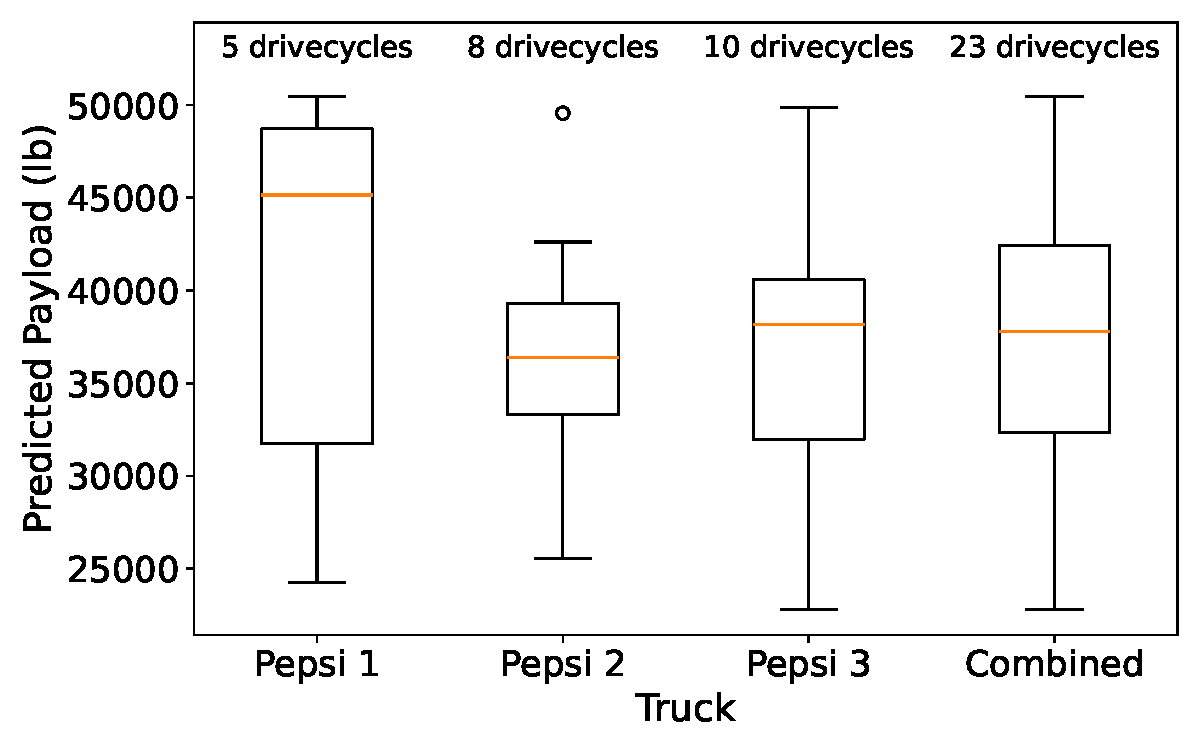
\includegraphics[width=\textwidth]{figures/payload_distribution.pdf}
        \caption{Payload}
        \label{fig:payload_distribution}
    \end{subfigure}
    \hfill
    \begin{subfigure}[b]{0.49\textwidth}
        \centering
        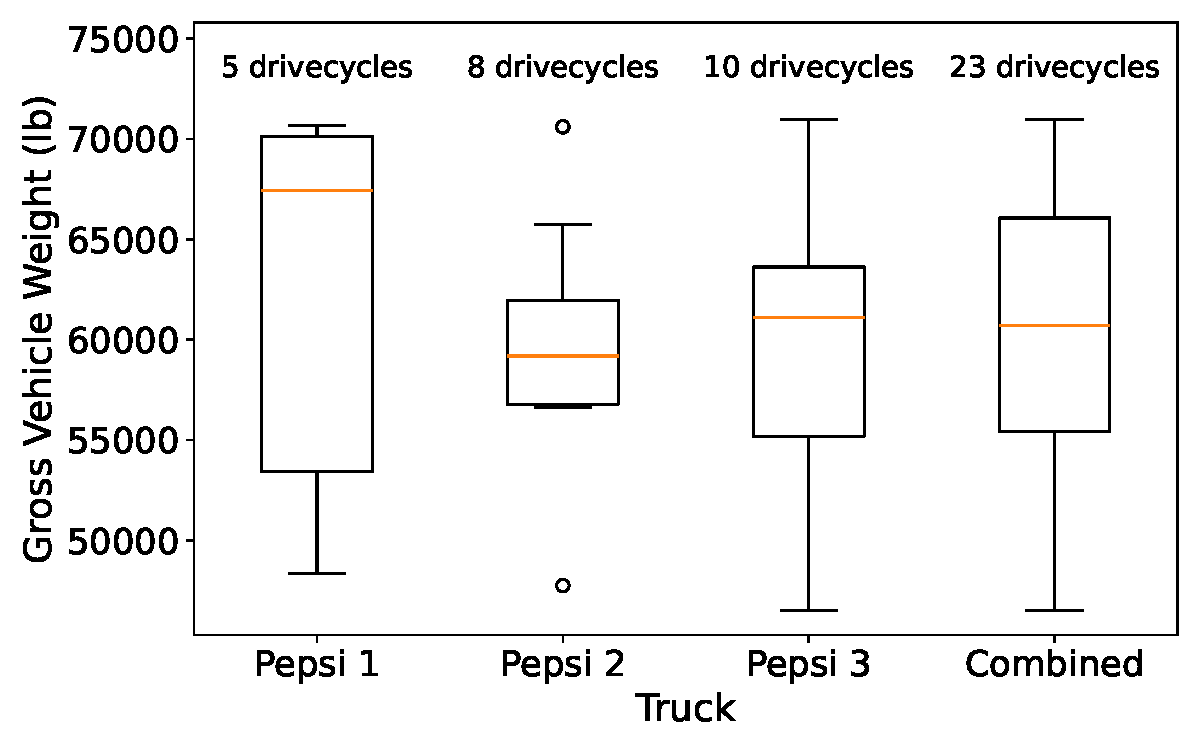
\includegraphics[width=\textwidth]{figures/gvw_distribution.pdf}
        \caption{Gross Vehicle Weight}
        \label{fig:gvw_distribution}
    \end{subfigure}
    \caption{Summary of payloads and gross vehicle weights evaluated for all drivecycles classified as linear in the NACFE data from the PepsiCo Tesla Semi pilot. The median of values for each truck is shown in orange, and boxes span the upper and lower quartiles. Whiskers extend to the minimum and maximum values, and outliers are shown as unfilled circles.}
    \label{fig:payload_gvw_distributions}
\end{figure}

\subsubsubsection{Average Linear Relationship Between Payload and Energy Economy}

As highlighted in Equation \ref{eq:energy_economy}, the energy economy of a given truck carrying a fixed payload will in general vary between drivecycles due to differences in truck speeds and road grades over the drivecycle. However, by calculating a weighted average of linear slopes and intercepts in Equation \ref{eq:energy_economy} over all drivecycles, we can estimate the linear relationship between the payload carried by a Semi truck and its average energy economy on the basis of the flat-terrain drivecycles carried out in the PepsiCo pilot. 

Figure \ref{fig:slope_intercept_distributions} summarizes the slopes and intercepts evaluated for drivecycles carried out by each truck. The slopes are consistent between trucks within one quartile. The y-intercepts are largely consistent. The small inconsistency in intercepts between Pepsi 1 and Pepsi 2 is considered reasonable given the limited statistics. 

\begin{figure}[H]
    \centering
    \begin{subfigure}[b]{0.49\textwidth}
        \centering
        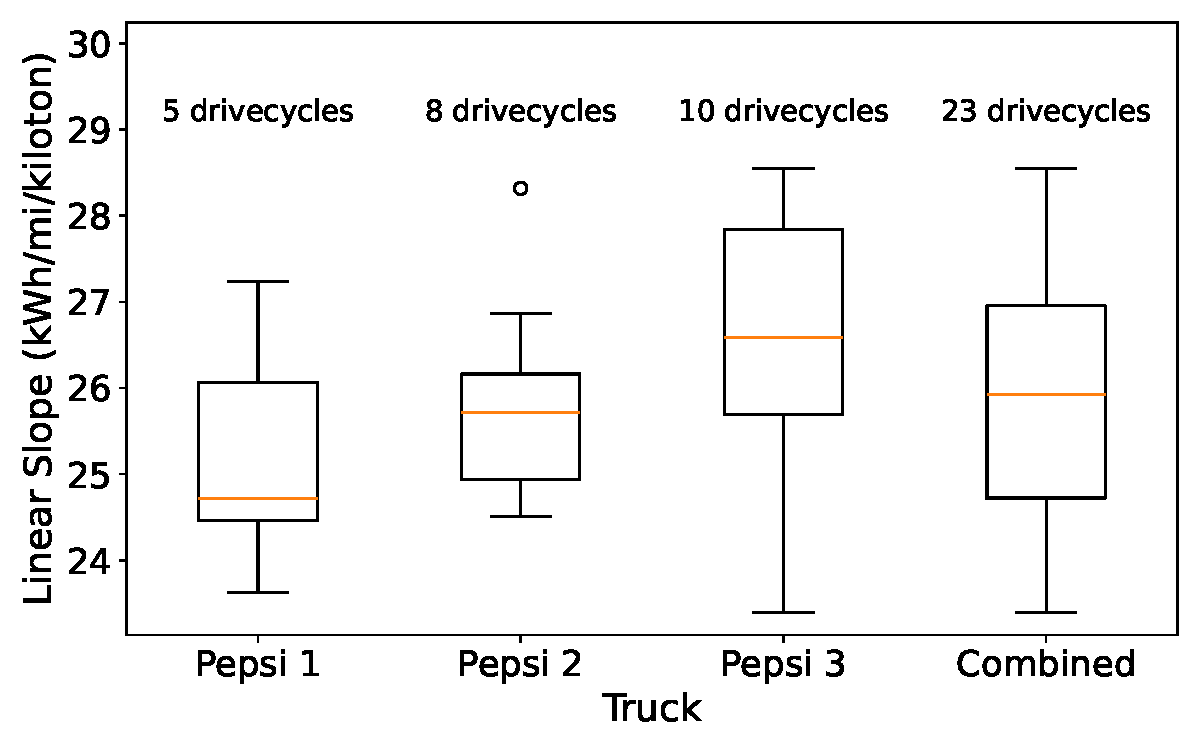
\includegraphics[width=\textwidth]{figures/slope_distribution.pdf}
        \caption{Slope}
        \label{fig:slope_distribution}
    \end{subfigure}
    \hfill
    \begin{subfigure}[b]{0.49\textwidth}
        \centering
        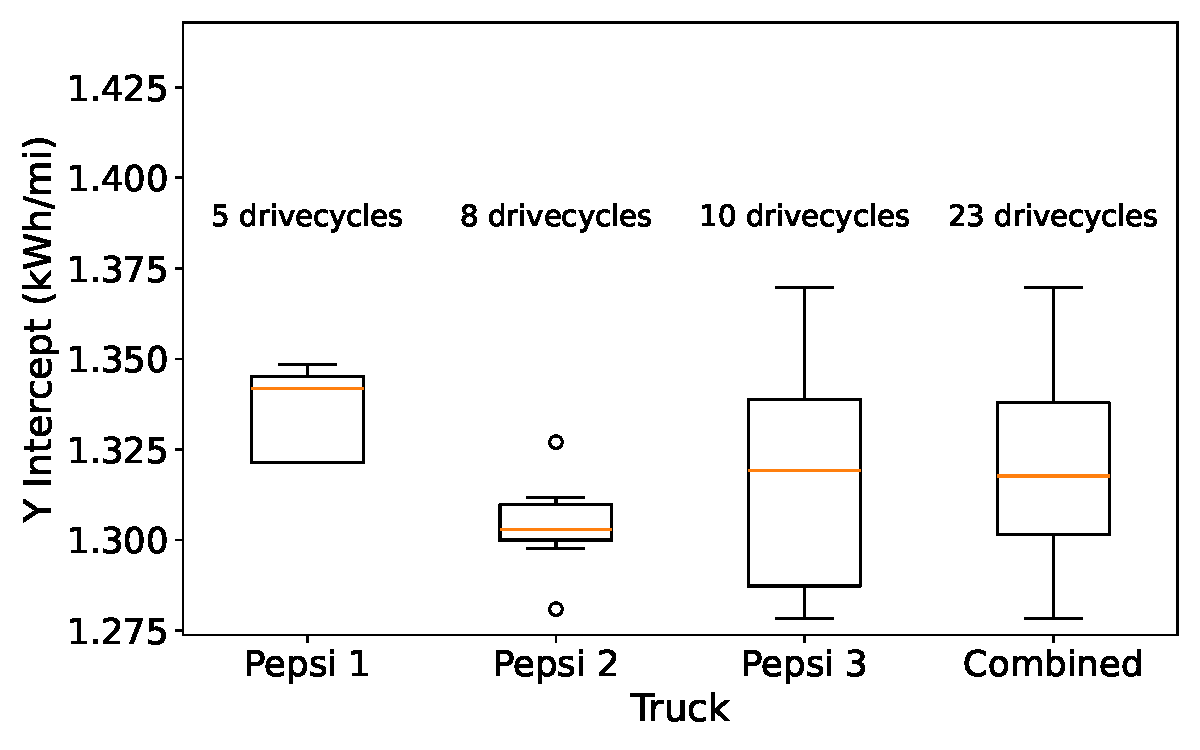
\includegraphics[width=\textwidth]{figures/intercept_distribution.pdf}
        \caption{Intercept}
        \label{fig:intercept_distribution}
    \end{subfigure}
    \caption{Summary of slopes and intercepts in Equation \ref{eq:energy_economy} evaluated for each drivecycle classified as linear (flat-terrain). The median of values for each truck is shown in orange, and boxes span the upper and lower quartiles. Whiskers extend to the minimum and maximum values, and outliers are shown as unfilled circles.}
    \label{fig:slope_intercept_distributions}
\end{figure}

Taking the average over all slopes and intercepts, the estimated linear relationship between payload and energy economy is shown in Figure \ref{fig:payload_vs_energy_economy_ev}. The uncertainty band is derived from the standard deviations of the slope and y intercept values, neglecting potential correlation. The energy economy is found to range from $\sim 1.4-2.0$ kWh/mile within the legal GVW range of 0-82,000 lb for EVs in California. This range is in good agreement with Tesla's advertised value of ``less than 2 kWh per mile" \cite{tesla_semi}. 

\begin{figure}[H]
        \centering
        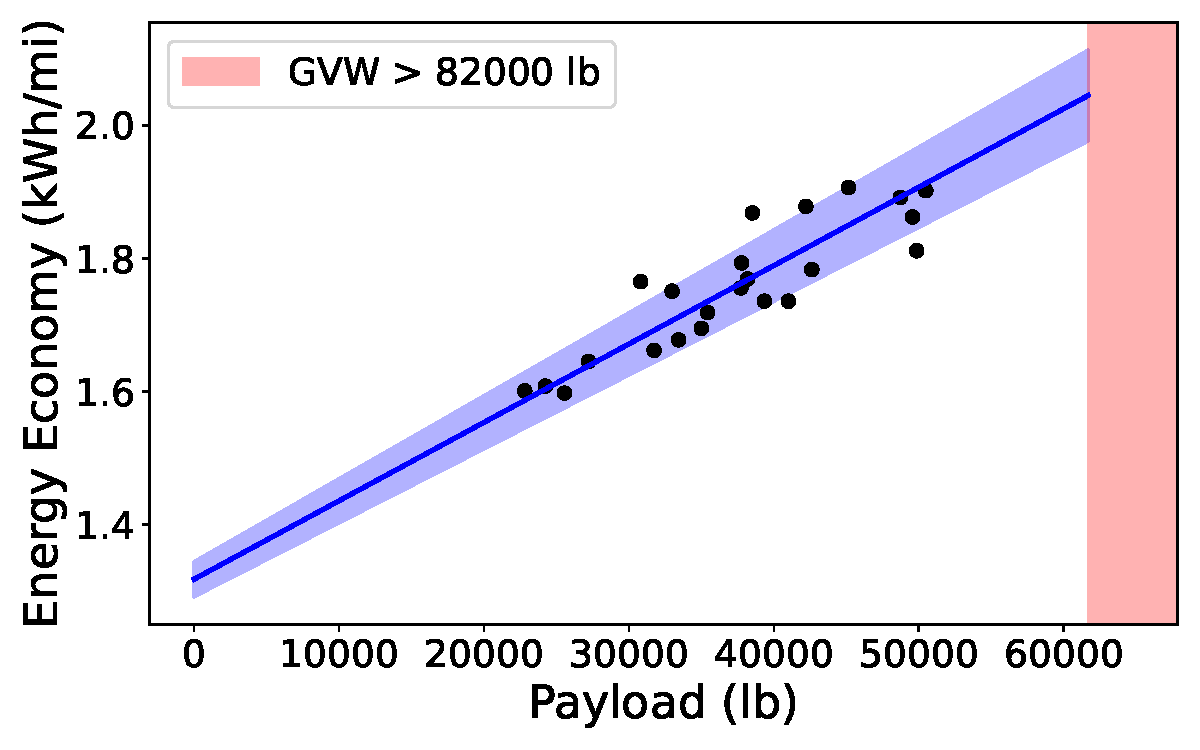
\includegraphics[width=0.7\textwidth]{figures/payload_vs_energy_economy_function_ev.pdf}
        \caption{Average linear relationship between energy economy and payload for the Tesla Semi, derived from drivecycles classified as ``linear" in the NACFE data from PepsiCo's Tesla Semi pilot. The uncertainty band is shown in blue, and values of energy economy and payload evaluated for individual drivecycles are shown with black circles. The red region represents payloads for which the GVW exceeds California's legal limit for EV trucks of 82,000 lb.}
        \label{fig:payload_vs_energy_economy_ev}
\end{figure}

\subsection{Adaptations to Model an Equivalent Diesel Truck}
\label{sec:diesel_adaptations}

The electric vehicle (EV) truck model was adapted to additionally evaluate the average energy economy with respect to payload of a diesel internal combustion truck whose non-powertrain specifications are equivalent to the Tesla Semi. To perform this adaptation, the evaluation of energy economy is modified relative to Ref. \cite{Sader_2023} as follows:

First, Equation 2 in Ref. \cite{Sader_2023} is modified to represent the power demand on the engine rather than the battery:

\begin{equation}
    \label{eq:power_demand_engine_pos}
    P_\text{engine}(t) = \frac{P_\text{wheel}(t)}{\eta_e\eta_t} + \frac{P_\text{aux}}{\eta_e} \quad \text{if }P_\text{wheel} \geq 0
\end{equation}

\begin{equation}
    \label{eq:power_demand_engine_neg}
    P_\text{engine}(t) = \frac{P_\text{aux}}{\eta_e\eta_t} \quad \text{if }P_\text{wheel} < 0
\end{equation}

\noindent where $\eta_e$ is the engine efficiency and $\eta_t$ is the transmission efficiency. Table \ref{tab:diesel_params} summarizes the engine and transmission efficiency, along with other diesel truck model parameters that differ from those used to simulate the Tesla Semi. The energy economy, evaluated with $P_\text{bat}$ substituted for $P_\text{engine}$ in Equation 4 of Ref. \cite{Sader_2023}, is converted from kWh/mile to gallons/mile using the lower heating value of low sulfur diesel \cite{afdc_fuel_properties} and inverted to obtain the fuel economy in miles/gallon. 

\begin{table}[H]
\centering
\begin{tabular}{P{3cm}P{2.5cm}P{2cm}P{7cm}} % Adjust the column widths as needed
\toprule % Thicker top line
\textbf{Parameter} & \textbf{Value for Diesel Truck} & \textbf{Value for EV Truck} & \textbf{Description} \\ 
\midrule % Midrule for under header
Maximum motor power & 370 kW & 942.9 kW & Rated power of 12L class 8 diesel engine simulated in \cite{Jones_et_al_2024}. \\
\midrule % Midrule for under header
Auxiliary motor power & 5 kW & 10 kW & Auxiliary power for class 8 diesel engine simulated in \cite{Jones_et_al_2024}. \\
\midrule % Midrule for under header
Engine efficiency $\eta_e$ & 0.421 & - & Brake thermal efficiency averaged over a full drivecycle for the ``world harmonized transient cycle" \cite{unece2007}, evaluated in Ref. \cite{icct2017hdv} for a present-day baseline heavy duty tractor-trailer. \\
\midrule % Midrule for under header
Transmission efficiency $\eta_t$ & 0.99 & - & Maximum transmission efficiency among present-day heavy duty tractor trailers, from Ref. \cite{icct2017hdv}. \\
\bottomrule % Thicker bottom line
\end{tabular}
\caption{Summary of parameters updated to simulate a diesel truck with non-powertrain specifications roughly equivalent to the Tesla Semi}
\label{tab:diesel_params}
\end{table}

The method outlined in Section \ref{sec:payload_evaluation} is used to evaluate an approximate linear relationship between energy economy and payload based on the NACFE drivecycles, with Equation \ref{eq:payload} updated to:

\begin{equation}
\label{eq:payload_diesel}
\text{Payload} = m - m_\text{truck, no battery}
\end{equation}

Figure \ref{fig:slope_intercept_distributions_diesel} summarizes the slopes and intercepts evaluated with Equation \ref{eq:energy_economy} for simulated diesel trucks, and Figure \ref{fig:payload_vs_energy_economy_diesel} shows the estimated inverse linear relationship between the payload carried by the diesel truck and its fuel economy, in miles per gallon (mpg). The fuel economy ranges from  $~\sim9-17$ mpg within the legal GVW range. This range is significantly above the average fuel economy of 6.6 mpg reported for heavy duty trucks in the U.S. by the Federal Higways Administration \cite{fhwa_2018}. However, it includes the 10.1 mpg attained by tractor-trailers equipped with state-of-the-art efficiency technologies during a NACFE Run on Less Efficiency demonstration in 2017 \cite{nacfe_run_2017}. This reflects the use of ``current best-in-class" efficiency parameters needed to simulate the performance of the Tesla Semi and its approximate diesel equivalent. As noted in Section \ref{sec:payload_evaluation}, even using the best-in-class parameters found in the literature, the performance of the simulated EV truck was found to be conservative in comparison to reports from Tesla. 

\begin{figure}[H]
    \centering
    \begin{subfigure}[b]{0.49\textwidth}
        \centering
        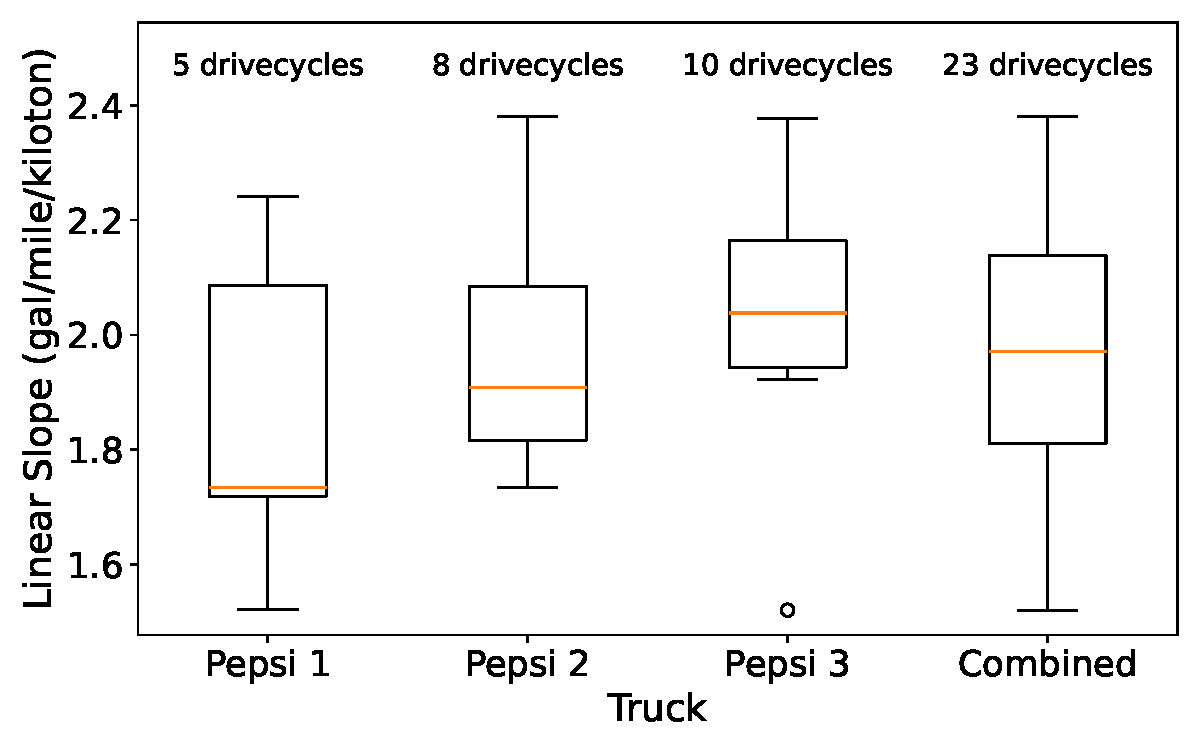
\includegraphics[width=\textwidth]{figures/slope_distribution_diesel.pdf}
        \caption{Slope}
        \label{fig:slope_distribution_diesel}
    \end{subfigure}
    \hfill
    \begin{subfigure}[b]{0.49\textwidth}
        \centering
        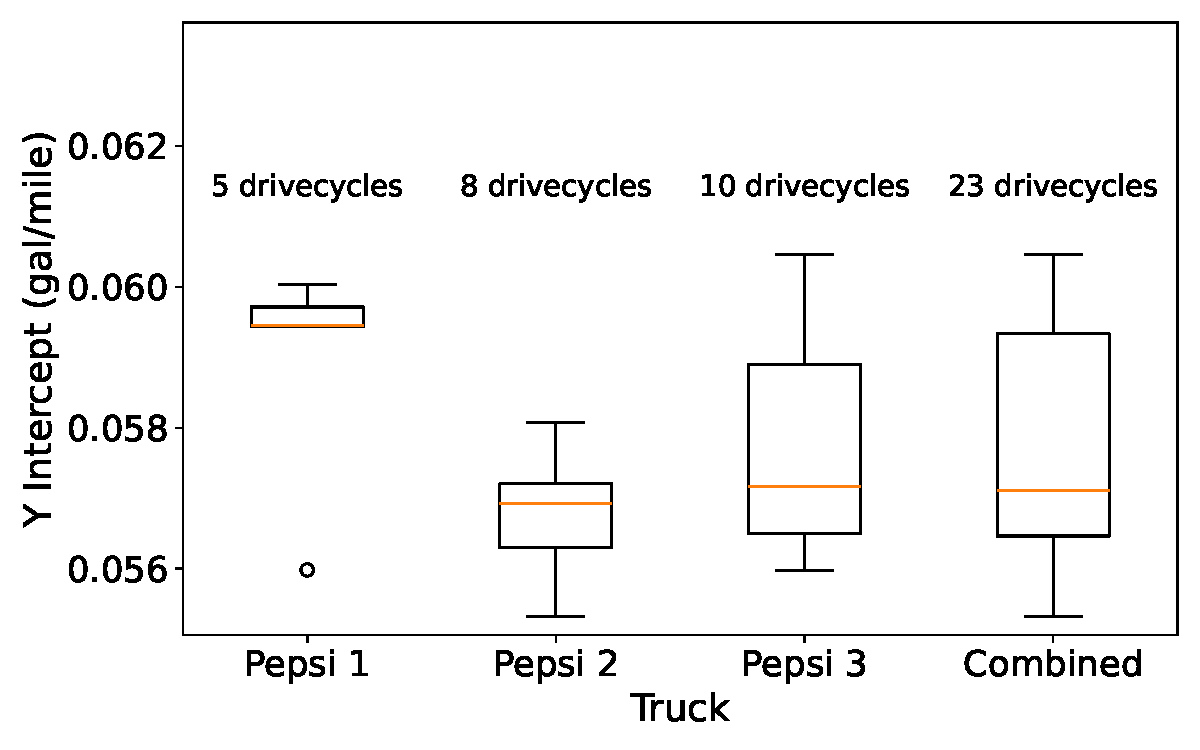
\includegraphics[width=\textwidth]{figures/intercept_distribution_diesel.pdf}
        \caption{Intercept}
        \label{fig:intercept_distribution_diesel}
    \end{subfigure}
    \caption{Summary of slopes and intercepts in Equation \ref{eq:energy_economy} evaluated for each drivecycle classified as linear (flat-terrain). The median of values for each truck is shown in orange, and boxes span the upper and lower quartiles. Whiskers extend to the minimum and maximum values, and outliers are shown as unfilled circles.}
    \label{fig:slope_intercept_distributions_diesel}
\end{figure}

\begin{figure}[H]
        \centering
        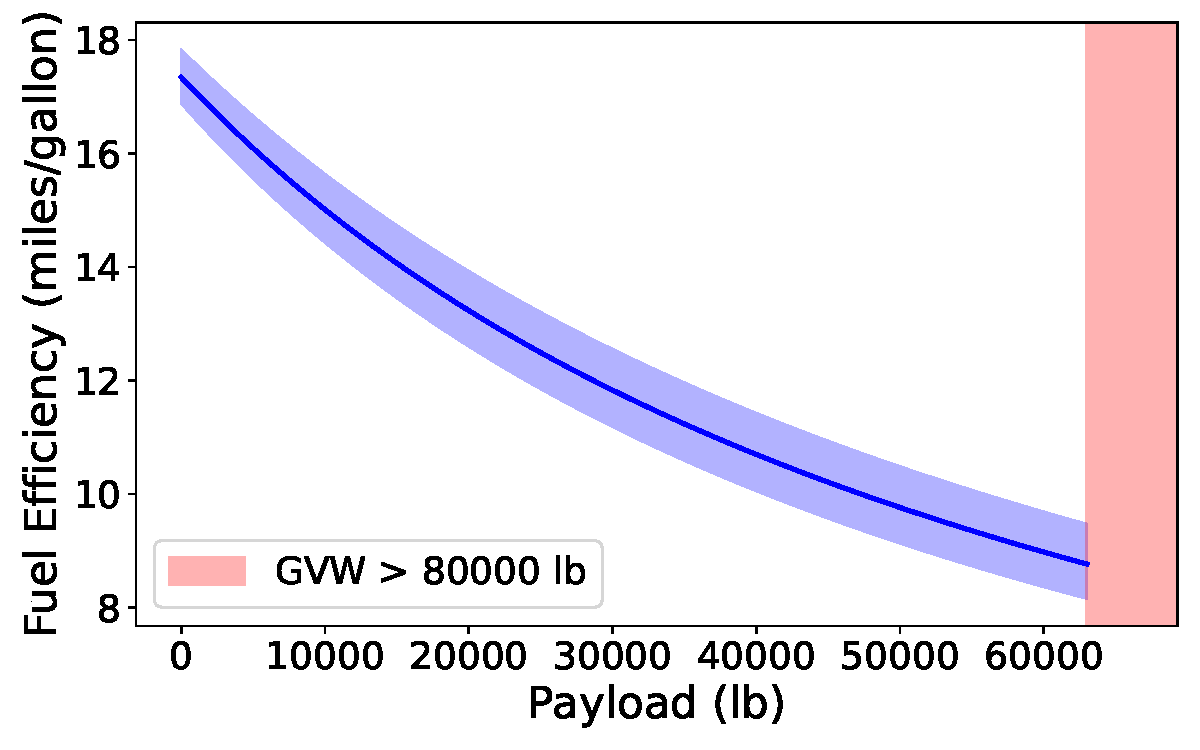
\includegraphics[width=0.7\textwidth]{figures/payload_vs_mileage_function_diesel.pdf}
        \caption{Average inverse linear relationship between fuel economy (mile per gallon) and payload for a diesel truck equivalent of the Tesla Semi, derived from drivecycles classified as ``linear" in the NACFE data from PepsiCo's Tesla Semi pilot. The uncertainty band is shown in blue. The red region represents payloads for which the GVW exceeds the U.S class 8 legal limit of 80,000 lb.}
        \label{fig:payload_vs_energy_economy_diesel}
\end{figure}

\subsection{Adaptations to Model Total Cost of Ownership and Lifecycle Emissions}

A major goal of integrating the model developed by Sader et al. \cite{Sader_2023} into the Geo-FTADS tool is to allow users to explore how the total cost of truck ownership and associated well-to-wheel emissions vary between different regions and operating profiles. The interactive features of the geospatial tool that support this exploration are introduced in Section \ref{sec:elec_price_emissions_intensity}. 

Here, we discuss the methodology involved in adding flexibility to the cost and emissions models described in Sections 2.3 and 2.4 of Sader et al. \cite{Sader_2023} to evaluate the costs and emissions visualized in the tool with respect to parameters that vary between different regions and operating profiles. This methodology is applied to the truck simulation discussed in Sections \ref{sec:semi_adaptations} and \ref{sec:diesel_adaptations}, which is adapted from the simulation in Ref. \cite{Sader_2023} to represent the Tesla Semi and an equivalent diesel truck.

Table \ref{tab:cost_emissions_parameters} summarizes the parameters that can be varied in the updated model displayed on the Geo-FTADS tool, and the following sections detail the modifications made for each parameter. 

\begin{table}[H]
\centering
\begin{tabular}{P{3cm}P{3cm}P{2.5cm}P{2cm}P{4cm}} % Adjust the column widths as needed
\toprule % Thicker top line
\textbf{Parameter} & \textbf{Range} & \textbf{Default Value} & \textbf{Source of Variation} & \textbf{Description} \\ 
\midrule % Midrule for under header
Average vehicle miles traveled (VMT) & [40,000 miles, 190,000 miles] & 100,000 miles & Operational profile & Average annual miles traveled by the truck over its lifetime. \\
\midrule % Midrule for under header
Average payload (lb) & [0, 50,000 lb] & 40,000 lb & Operational profile & Average payload carried by truck. \\
\midrule % Midrule for under header
Maximum charging power (kW) & [100, 400] & 400 kW & Operational profile & Maximum power used for truck charging. \\
\midrule % Midrule for under header
Average state electricity price (US cents/kWh) & [7.77, 30.88] & None (defined by state) & Operating region & Average price of electricity by state. \\
\midrule % Midrule for under header
Average demand charge (USD/kW) & [0.0, 90.37] & None (defined by state) & Operating region & Maximum historical demand charge in a given region. \\
\midrule % Midrule for under header
Diesel price (USD/gallon) & [3.8, 5.1] & None (defined by state) & Operating region & Diesel price by state. \\
\midrule % Midrule for under header
Grid emission intensity (lb/MWh) &  [13, 1960] & None (defined by state) & Operating region & Average grid emission intensity, reported either by state or by balancing authority. \\
\bottomrule % Thicker bottom line
\end{tabular}
\caption{Input parameters to the total cost of ownership and emissions model, modified from Ref \cite{Sader_2023}.}
\label{tab:cost_emissions_parameters}
\end{table}

\subsubsection{Payload and vehicle miles traveled}

In the original model \cite{Sader_2023}, the payload is input as a distribution based on real-world data \cite{zabelsky2002economic} for the U.S. fleet. The vehicle miles traveled (VMT) is obtained from Ref. \cite{osti_1780970} as an average value for each year of the truck's assumed 10-year lifetime, resulting in a distribution of VMT over 10 years.  

For a given average value of these parameters, the payload and VMT distributions input to the model are scaled by a constant multiple such that the average value of the distribution matches the desired value. This process is illustrated in Figure \ref{fig:VMT_payload_scaling}.

\begin{figure}[H]
    \centering
    \begin{subfigure}[b]{0.49\textwidth}
        \centering
        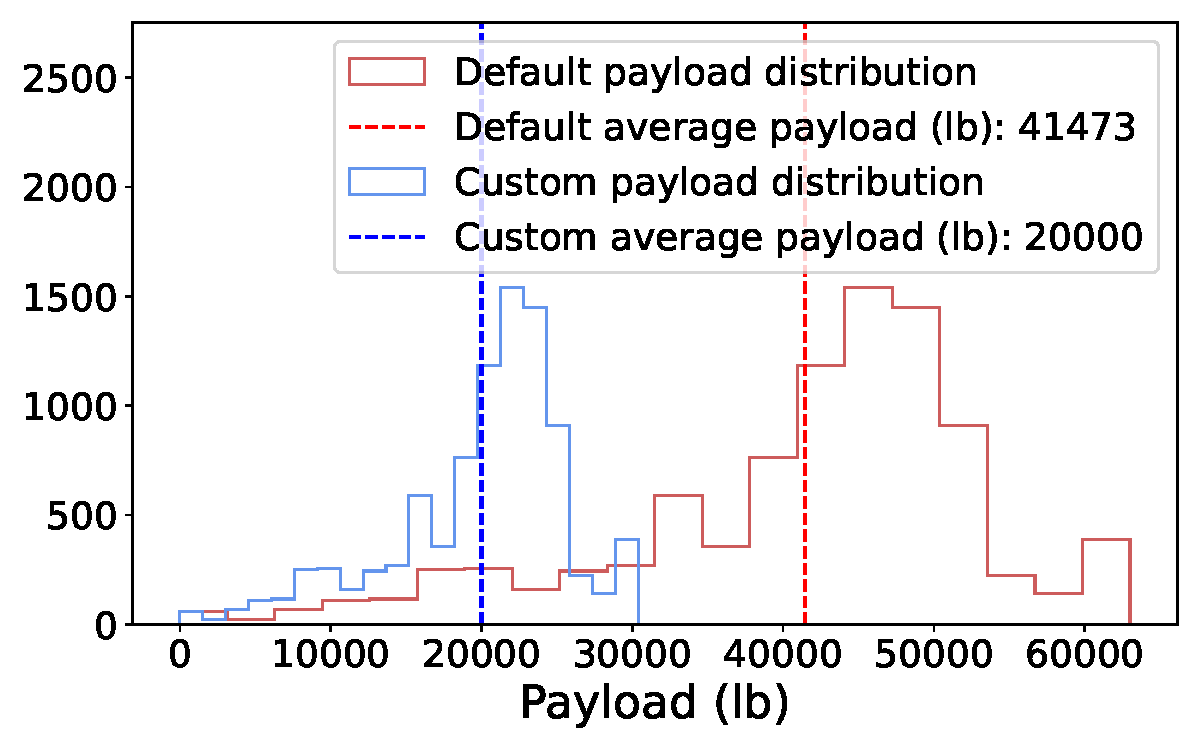
\includegraphics[width=\textwidth]{figures/payload_distribution_average_20000lb.pdf}
        \caption{Payload}
        \label{fig:payload_distribution}
    \end{subfigure}
    \hfill
    \begin{subfigure}[b]{0.49\textwidth}
        \centering
        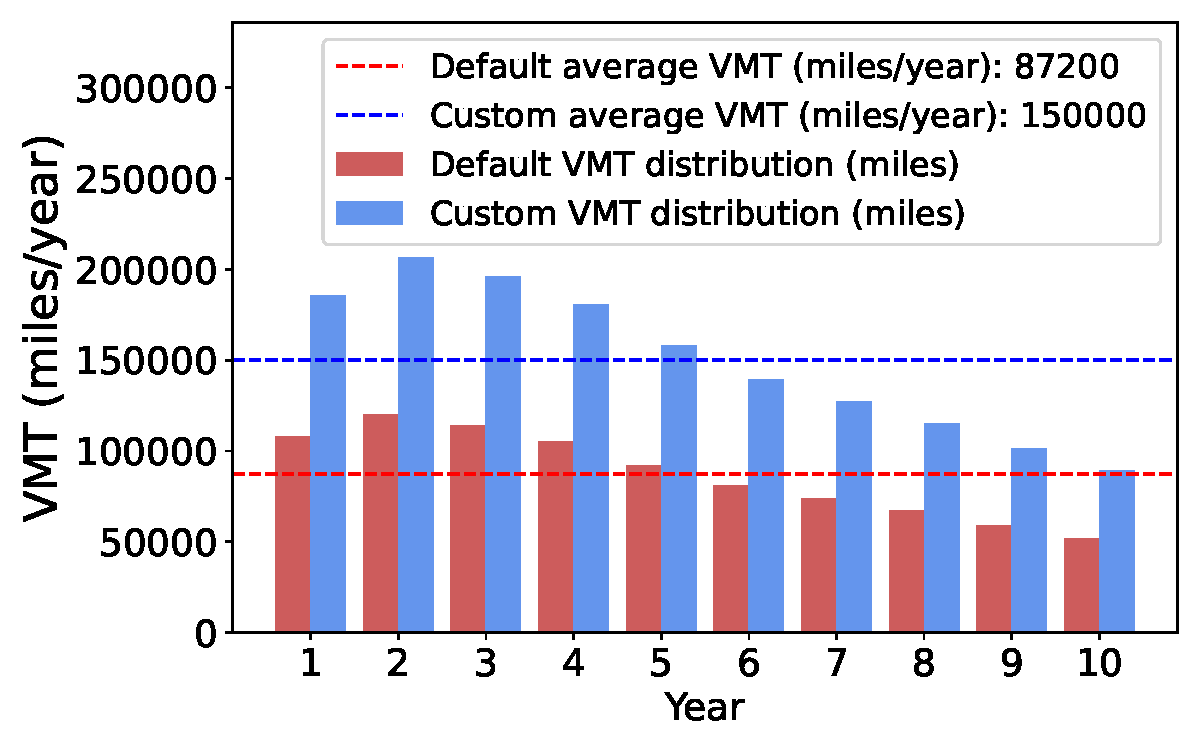
\includegraphics[width=\textwidth]{figures/VMT_distribution_average_150000.pdf}
        \caption{Vehicle Miles Traveled (VMT)}
        \label{fig:VMT_distribution_average_150000}
    \end{subfigure}
    \caption{Left: The payload distribution is scaled from its default average of 41,473 lb to a custom input average of 20,000. Right: The distribution of average vehicle miles traveled (VMT) over a 10-year truck lifetime is scaled from its 10-year average value of 87,200 miles/year to a custom average of 150,000 miles/year.}
    \label{fig:VMT_payload_scaling}
\end{figure}

\subsubsection{Electricity Cost}

As discussed in Section 2.4.4 of Ref. \cite{Sader_2023}, the cost of electricity used to calculate the total cost of ownership accounts for the capital cost $C_\text{CAPEX}$ of purchasing and installing charging infrastructure, as well as fixed monthly charges from the utility $C_\text{monthly fixed charge from utility}$, the electricity price per kWh $C_\text{energy charge from utility}$, and the monthly utility demand charge $C_\text{demand charge from utility}$. It varies with the following parameters listed in Table \ref{tab:cost_emissions_parameters}:

\begin{itemize}
    \item The user-specified average of the VMT distribution $VMT(y)$ over all years $y$ of the truck's lifetime
    \item The state electricity price $C_\text{energy charge from utility}$, introduced in Section \ref{sec:elec_price_emissions_intensity}.
    \item The monthly utility demand charge $C_\text{demand charge from utility}$, also introduced in Section \ref{sec:elec_price_emissions_intensity}.
\end{itemize}

During each year $y$ of the truck's assumed 10-year lifetime, the overall cost of electricity per kWh of battery charging energy is given by:

\begin{equation}
    \label{eq:total_electricity_cost}
    \begin{aligned}
    C_\text{total per kWh}(y) = & \ C_\text{CAPEX per kWh} + C_\text{fixed charge per kWh}(y) \\
    & + C_\text{energy charge per kWh} + C_\text{demand charge per kWh}(y)
    \end{aligned}
\end{equation}

\noindent where $C_\text{energy charge}$, obtained with Equation 19 in Ref. \cite{Sader_2023} accounts for the efficiency of the charging equipment. The CAPEX, fixed montly utility charge, and monthly demand charge are normalized over the relevant time periods to obtain a cost per kWh. Here, we show how Equations 16, 17, 18, and 20 in Ref. \cite{Sader_2023} are re-parameterized to explicitly perform this normalization with respect to $VMT(y)$. 

The CAPEX per kWh is evaluated as follows:

\begin{equation}
    \label{eq:capex}
    C_\text{CAPEX per kWh} = \frac{C_\text{CAPEX}\times(1+d)^{t_\text{life cycle}}}{E_\text{total}}
\end{equation}

\noindent where $E_\text{total}$, the total energy consumed over the truck's lifetime to charge its battery is given by:

\begin{equation}
    \label{eq:E_total}
    E_\text{total} = \sum_{y=1}^{10} VMT(y) \times (\text{energy economy})
\end{equation}

The fixed monthly utility and demand charges are given by:

\begin{equation}
    \label{eq:monthly_charge}
    C_\text{fixed charge per kWh}(y) = \frac{C_\text{monthly fixed charge from utility}}{E_\text{charge, monthly}(y)}
\end{equation}

and
\begin{equation}
    \label{eq:monthly_charge}
    C_\text{demand charge per kWh}(y) = \frac{P_\text{charger}\times C_\text{demand charge from utility}}{E_\text{charge, monthly}(y)}
\end{equation}

\noindent where $P_\text{charger}$ is the power used for truck charging in kW, and $E_\text{charge, month}(y)$ is the amount of energy used to charge the battery during an average month in year $y$, given by:

\begin{equation}
    \label{eq:e_month}
    E_\text{charge, monthly} = \frac{VMT(y) \times (\text{energy economy)}}{12\text{ months/year}}
\end{equation}

Figure \ref{fig:energy_cost_by_year} shows the average energy cost calculated for each year of a truck's lifetime, assuming that charging takes place at a maximum charging power of 400 kW in California, which has an average state electricity price of 19.2 cents/kWh based on EIA data \cite{EIA_2024} and maximum demand charge of 13.4 \$/kW. The total unit cost generally increases over time because the vehicle travels fewer miles over which to amortize the monthly utility demand charge and fixed costs. 

\begin{figure}[H]
        \centering
        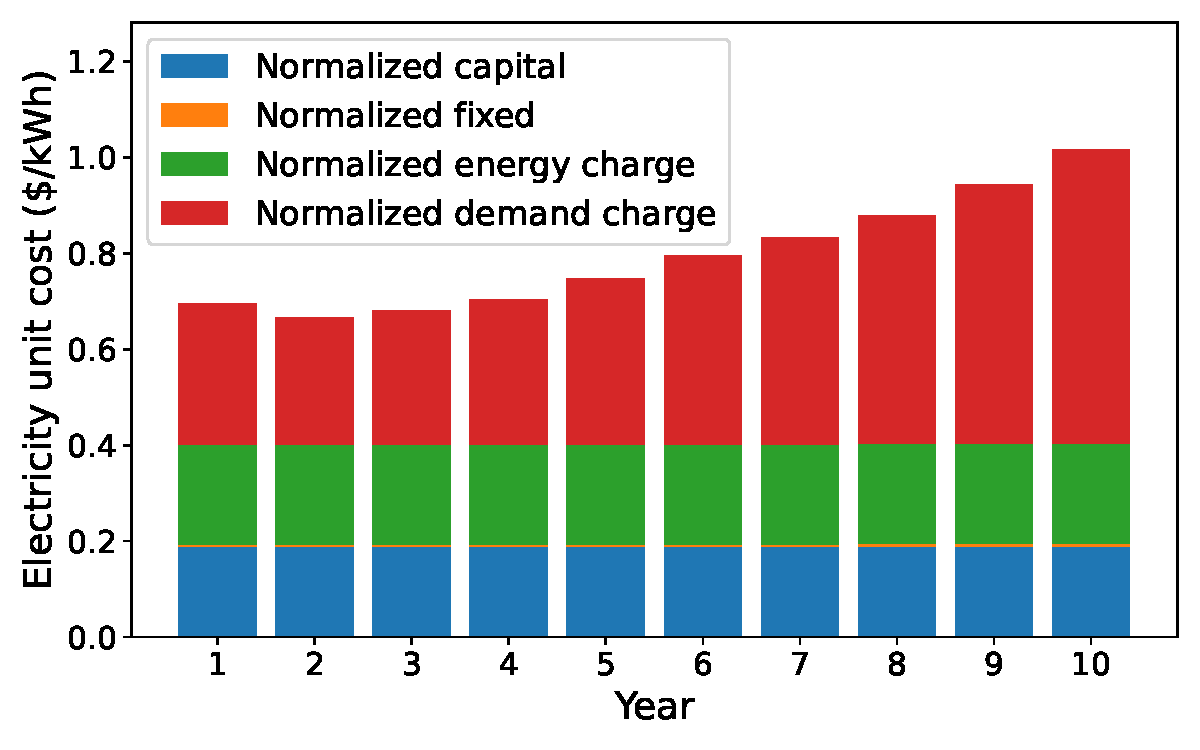
\includegraphics[width=0.7\textwidth]{figures/electricity_unit_price_CA.pdf}
        \caption{Average total electricity price per kWh calculated for each year of a truck's assumed 10-year life using Equations \ref{eq:total_electricity_cost} to \ref{eq:e_month} for a truck charging in California at a maximum charging power of 400 kW. } 
        \label{fig:energy_cost_by_year}
\end{figure}

\subsubsection{Battery replacements}
\label{sec:battery_replacement}

The number of battery replacements expected over the truck's lifetime is fixed to 1 for NMC batteries in Ref. \cite{Sader_2023}. Here, we instead estimate the number of battery replacements based on the VMT of the truck, assuming that the battery will need to be replaced every 1,000 equivalent full cycles. 

A 1,000-cycle battery life is conservatively chosen based on a study by Ecker et al. \cite{Ecker_2014} that quantifies various measures of battery health for NMC batteries, including normalized battery capacity, with respect to the number of full charge-discharge cycles carried out at a current of 1C and a temperature of 35$^{\circ}$C under various charging conditions. Based on the NACFE pilot data \cite{NACFE_2023}, the conditions under which the batteries were charged in the pilots, summarized in Table \ref{tab:battery_charging_stats}, most closely match the experimental conditions in Ref. \cite{Ecker_2014} in which the battery is charged from 25-75\%. Under these conditions, the battery capacity is found to reach 80\% after $\sim$1,200 cycles, following which it drops precipitously. 

In addition to being $\sim$20\% below the $\sim$1,200-cycle failure point observed in Ref. \cite{Ecker_2014}, the choice of 1,000 equivalent full cycles for the lifetime of an NMC EV battery operated approximately under the NACFE pilot conditions is considered conservative for two reasons. First, as shown in Table \ref{tab:battery_charging_stats}, the battery was on average charged at a C-value of 0.41, well below the $C=1$ used in the study. Second, while the battery discharges at 1C in Ref. \cite{Ecker_2014}, electric vehicle batteries generally discharge at a much slower rate as the vehicle is being driven. 

\begin{table}[H]
\centering
\begin{tabular}{P{4cm}P{4cm}P{4cm}} % Adjust the column widths as needed
\toprule % Thicker top line
\textbf{Parameter} & \textbf{Average over Charging Events} & \textbf{Standard Deviation over Charging Events} \\ 
\midrule % Midrule for under header
Minimum State of Charge (\%) & 36 & 27 \\
\midrule % Midrule for under header
Maximum State of Charge (\%) & 81 & 25 \\
\midrule % Midrule for under header
Depth of Discharge (\%) & 46 & 30 \\
\midrule % Midrule for under header
Average Charging Power (kW) & 340 & 214 \\
\midrule % Midrule for under header
C-value (h$^{-1}$) & 0.41 & 0.26 \\
\bottomrule % Thicker bottom line
\end{tabular}
\caption{Summary of conditions under which the Tesla Semi batteries were recharged in the PepsiCo pilot carried out during the NACFE Run on Less pilot \cite{NACFE_2023}.}
\label{tab:battery_charging_stats}
\end{table}

Based on a 1,000-cycle battery life, the number of battery replacements is calculated as follows:

\begin{equation}
    \label{eq:battery_replacements}
    \text{Battery replacements} = \text{floor}\Bigg(\frac{E_\text{total}}{E_\text{bat} \times 1000 \text{ cycles / battery life}}\Bigg)
\end{equation}

\noindent where $E_\text{bat}=825$ kWh, from Table \ref{tab:battery_capacity_summary}, is the average battery capacity evaluated over all three trucks involved in the NACFE pilot. $E_\text{total}$, which relates to the yearly VMT distribution according to Equation \ref{eq:E_total}, is the total energy consumed by the EV truck battery over the lifetime of the truck. 

Figure \ref{fig:battery_replacements} shows the number of battery replacements as a function of the average VMT for a truck carrying the default average payload of 40,000 lb.

\begin{figure}[H]
        \centering
        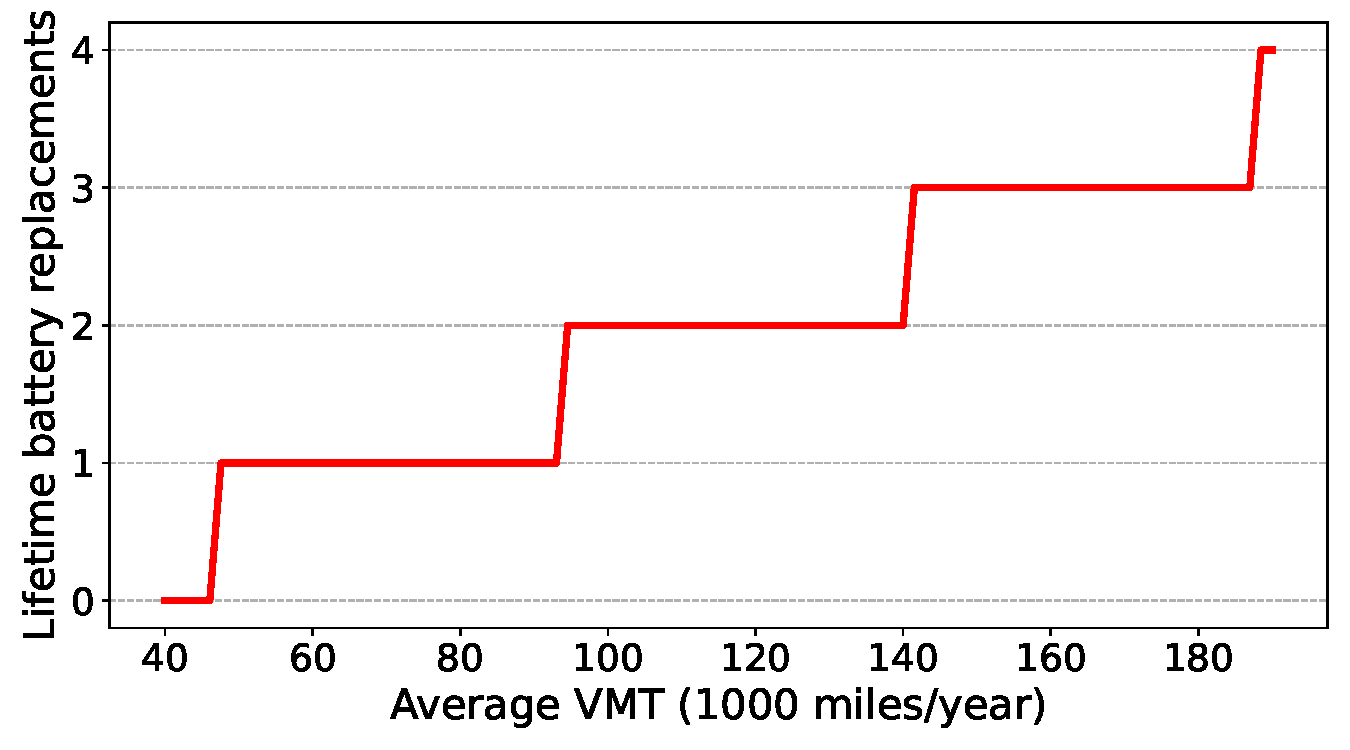
\includegraphics[width=0.7\textwidth]{figures/battery_replacements_vs_VMT_payload40000.pdf}
        \caption{Number of NMC battery replacements as a function of average VMT}
        \label{fig:battery_replacements}
\end{figure}

\subsubsection{Diesel price}

The diesel price for each state is estimated by averaging historical diesel prices over the last 5 years, adjusting historical prices for inflation using the U.S urban consumer price index \cite{cpi_2024}. The historical diesel prices are obtained from the Energy Information Administration \cite{eia2024gasdiesel}, and organized into five Petroleum Administration for Defense Districts (PADDs). The diesel price determined for each state depends on the PADD region in which the state is located.

\subsubsection{Grid emission intensity}

The average CO$_2$ equivalent emission intensity is obtained for 2022 either by balancing authority or by state from the eGRID database \cite{eGRID_2022}. Within a given state or balancing authority, the emission intensity is assumed to follow the same shape of exponential decay over time relative to its 2022 value as the fit to EIA projections evaluated in Ref. \cite{Sader_2023} for the average U.S. emission intensity. Figure \ref{fig:emission_intensity_exp} compares the projected carbon intensity of the WECC California balancing authority with the average U.S. intensity for a 10-year truck lifetime from 2024 to 2033. 

\begin{figure}[H]
        \centering
        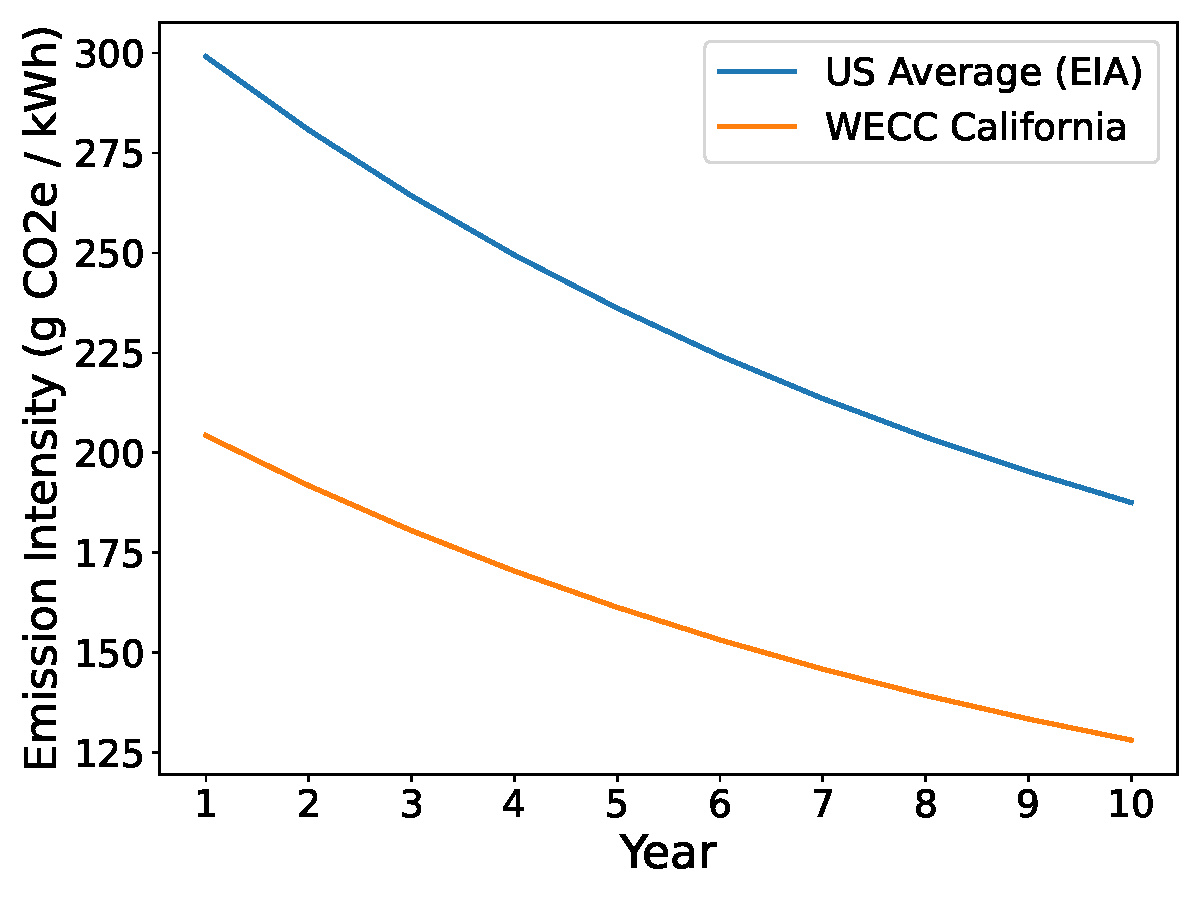
\includegraphics[width=0.7\textwidth]{figures/grid_emission_intensity_projection_CAMX.pdf}
        \caption{Projected emission intensity of the WECC California balancing authority grid over a 10-year truck lifetime from 2024-2033, compared with the projected average U.S. grid over the same time period.}
        \label{fig:emission_intensity_exp}
\end{figure}

\subsection{Total Cost of Ownership and Emissions}

With the model modifications and parameterization described in the above sections, the well-to-wheel emissions per mile of operating an EV truck calibrated to the Tesla Semi, including battery manufacturing and operation, are evaluated following Equations 8-10 in Ref. \cite{Sader_2023}. Figure \ref{fig:lifecycle_emissions} shows the resulting variation in emissions by state, using the default values of VMT, payload, and maximum charging power listed in Table \ref{tab:cost_emissions_parameters}. Figure \ref{fig:emissions_breakdown} shows the breakdown of well-to-wheel emissions per miles traveled into battery manufacturing and elecricity generation for several sample states, with model parameters set to their defaults in Table \ref{tab:cost_emissions_parameters}.

The total cost of EV truck ownership is calculated using Equation 21 in Ref. \cite{Sader_2023}, excluding the term $C_\text{GHG}\times\text{GHG}_\text{per mile}$ that quantifies the cost to society of CO$_2$ equivalent emissions. Table \ref{tab:tco_input_params} summarizes the model inputs used to estimate the total cost of ownership, both for an EV truck calibrated to the Tesla Semi and for an equivalent diesel truck. 

Figure \ref{fig:costs_breakdown} shows the breakdown of costs into capital costs, labor, electricity and other operating costs (``Other OPEX") for several sample states, with model parameters set to their defaults in Table \ref{tab:cost_emissions_parameters}. The cost breakdown in Figure \ref{fig:costs_breakdown} is shown both for electric vehicles and diesel trucks, and Section \ref{sec:tco_diesel} provides additional details of how these costs are evaluated for diesel trucks. Figure \ref{fig:ev_tco_map} shows how the total cost of EV truck ownership is visualized across U.S. states with the Geo-FTADS tool for the default model parameters. 

\begin{figure}[H]
    \centering
    \begin{subfigure}[b]{0.49\textwidth}
        \centering
        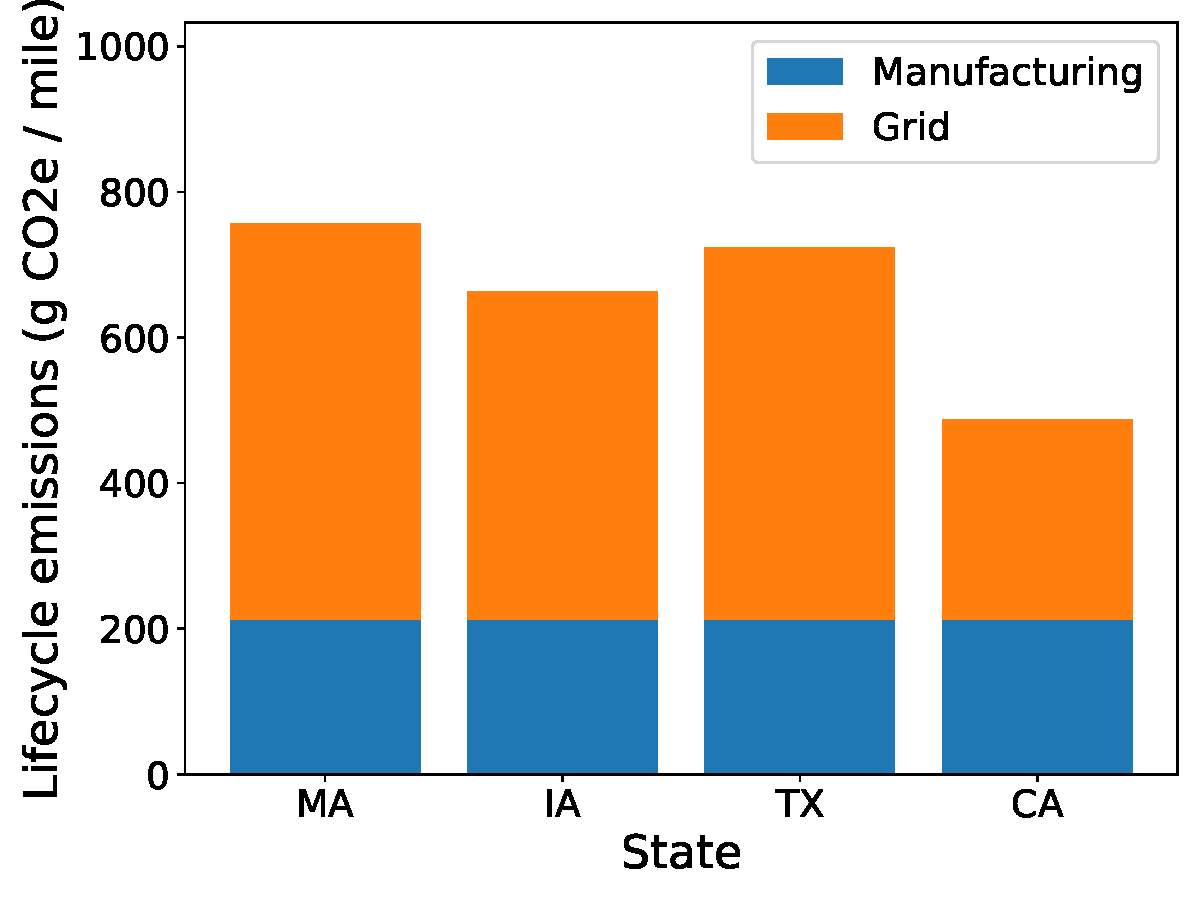
\includegraphics[width=\textwidth]{figures/emissions_per_mile.pdf}
        \caption{Emissions per mile}
        \label{fig:emissions_breakdown}
    \end{subfigure}
    \hfill
    \begin{subfigure}[b]{0.49\textwidth}
        \centering
        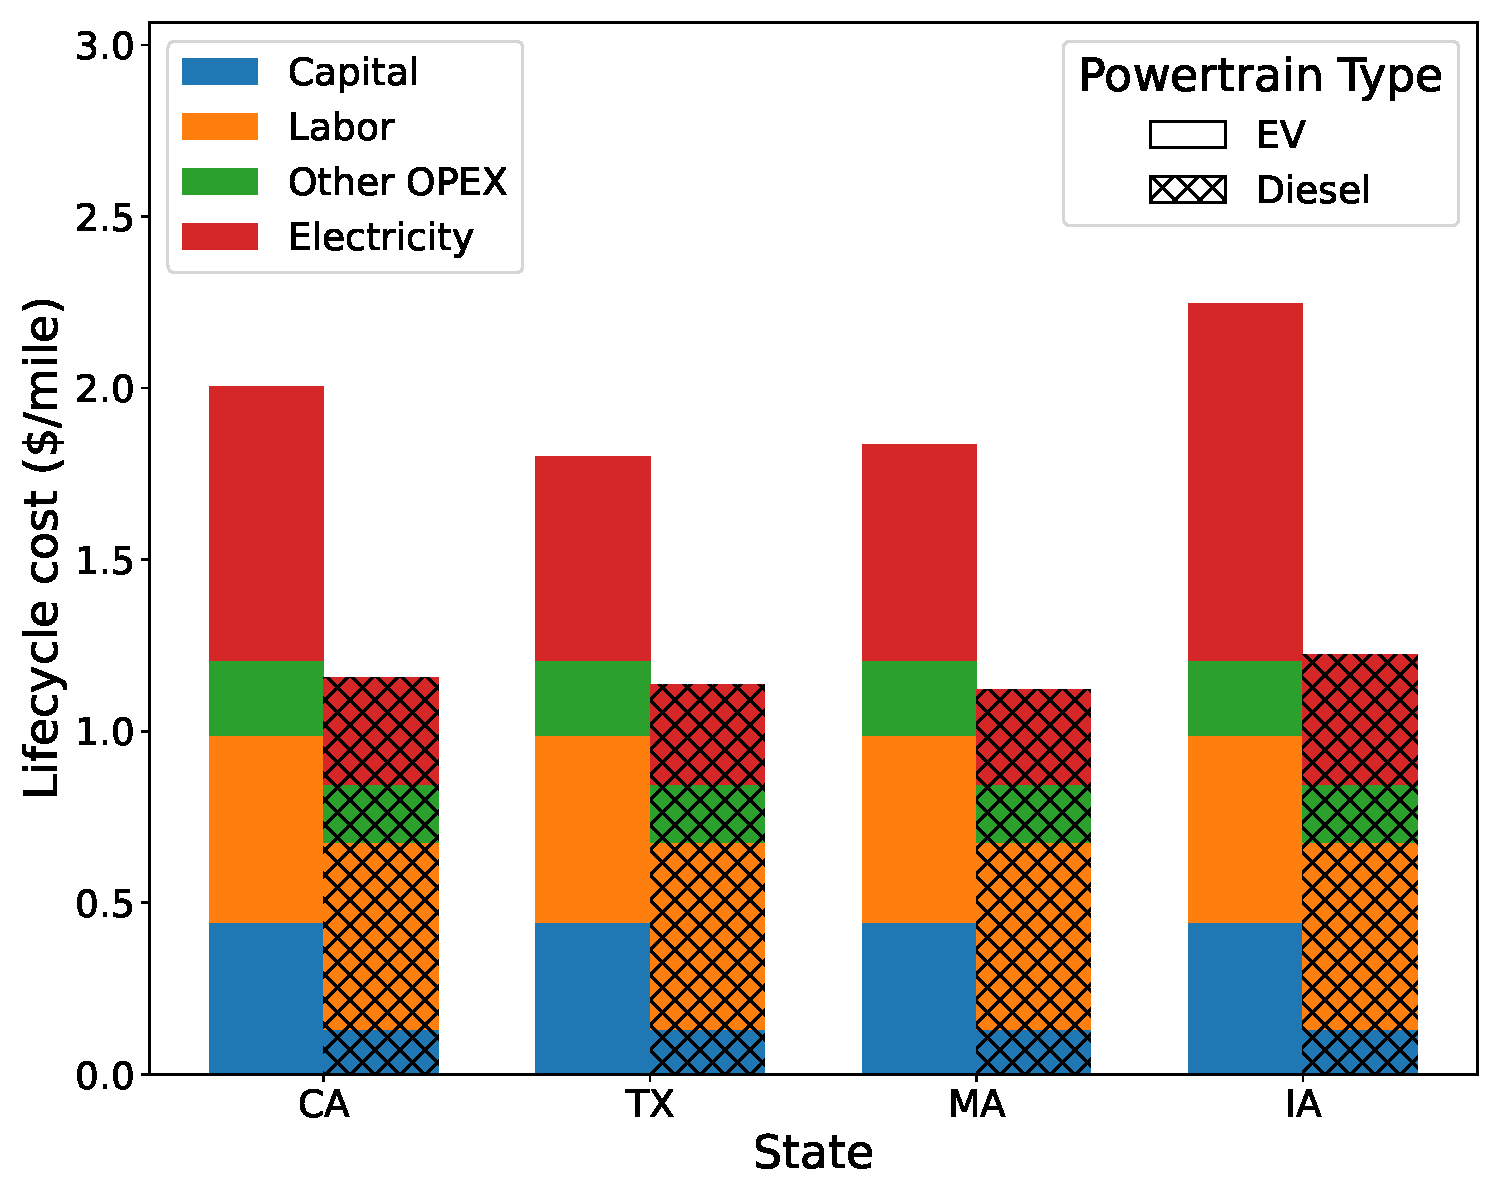
\includegraphics[width=\textwidth]{figures/costs_per_mile.pdf}
        \caption{Cost per mile}
        \label{fig:costs_breakdown}
    \end{subfigure}
    \caption{Breakdown of lifetime emissions (left) and costs (right) per mile for several sample states, with model parameters set to their default values in Table \ref{tab:cost_emissions_parameters}. The costs per mile in the right-hand plot are shown for both EV and diesel trucks for comparison.}.
    \label{fig:cost_emission_breakdowns}
\end{figure}

\begin{table}[H]
\centering
\begin{tabular}{P{3.5cm}P{2cm}P{1.5cm}P{1.5cm}P{2cm}P{5cm}}
\toprule % Thicker top line
\textbf{Cost Input} & \textbf{Cost Component} & \textbf{Value} & \textbf{Used for EV TCO} & \textbf{Used for Diesel TCO} & \textbf{Data Source} \\ 
\midrule % Midrule for under header
Glider (USD) & Capital & 95000 & \greencheck & \greencheck & Obtained from Ref. \cite{Jones_et_al_2024} \\
\midrule % Midrule for under header
Labor (USD/mile) & Labor & 0.69 & \greencheck & \greencheck & 2019 value for U.S. Trucking from Ref. \cite{atri2020operational} \\
\midrule % Midrule for under header
Tolls (USD/mile) & Other OPEX & 0.03 & \greencheck & \greencheck &  2019 value for U.S. Trucking from Ref. \cite{atri2020operational} \\
\midrule % Midrule for under header
Permits and licenses (USD/mile) & Other OPEX & 0.02 & \greencheck & \greencheck &  2019 value for U.S. Trucking from Ref. \cite{atri2020operational} \\
\midrule % Midrule for under header
EV truck insurance (USD/mile) & Other OPEX & 0.198 & \greencheck & \greencheck & Obtained from Ref. \cite{Sader_2023} \\
\midrule % Midrule for under header
Diesel truck insurance (USD/mile) & Other OPEX & 0.07 & \redx & \greencheck & 2019 value for U.S. Trucking from Ref. \cite{atri2020operational} \\
\midrule % Midrule for under header
Motor and inverter (USD/kW) & Capital & 77 & \greencheck & \redx & Data source: Cost of electric drive unit estimated for 2020 by Ref. \cite{icct2023cost} \\
\midrule % Midrule for under header
DC-DC converter (USD/kW) & Capital & 90 & \greencheck & \redx & Data source: Middle of 60-120 USD/kW estimate in Ref. \cite{icct2022etruck} \\
\midrule % Midrule for under header
NMC battery (USD/kWh) & Capital & 137 & \greencheck & \redx & 2020 cost of NMC batteries from Ref. \cite{Mauler_et_al_2021} \\
\midrule % Midrule for under header
Diesel engine (USD/kW) & Capital & 34.62 & \redx & \greencheck & Obtained from Ref. \cite{Jones_et_al_2024} \\
\midrule % Midrule for under header
Transmission (USD) & Capital & 10250 & \redx & \greencheck & Obtained from Ref. \cite{Jones_et_al_2024} \\
\midrule % Midrule for under header
Fuel Tank (USD) & Capital & 2100 & \redx & \greencheck & Obtained from Ref. \cite{icct2017zero} \\
\midrule % Midrule for under header
Aftertreatment (USD) & Capital & 5782 & \redx & \greencheck & Obtained from Ref. \cite{Jones_et_al_2024} \\
\midrule % Midrule for under header
Waste heat recovery system (USD) & Capital & 5900 & \redx & \greencheck & Obtained from Ref. \cite{Jones_et_al_2024} \\
\bottomrule % Thicker bottom line
\end{tabular}
\caption{Summary of cost parameters that are input to the TCO calculation for a diesel truck equivalent to the Tesla Semi.}
\label{tab:tco_input_params}
\end{table}

\subsubsection{Total cost of Ownership for Diesel Truck}
\label{sec:tco_diesel}

The total cost of ownership of diesel trucks is calculated following an equivalent methodology to that used for electric vehicle (EV) trucks in Ref. \cite{Sader_2023}, using the adapted diesel truck model presented in Section \ref{sec:diesel_adaptations} with some modifications to the capital and operating costs summarized in Table \ref{tab:tco_input_params}. Well-to-wheel emissions per mile have not yet been evaluated for diesel trucks in this framework. 

The fuel operating costs (Fuel OPEX) are evaluated for the diesel truck based on the diesel price and the fuel economy in mpg:

\begin{equation}
    \label{eq:diesel_opex}
    \text{Diesel Fuel OPEX (USD/mile)} = \frac{\text{diesel price (USD/gal)}}{\text{Fuel economy (mpg)}}
\end{equation}

Figure \ref{fig:costs_breakdown} compares the costs per mile for diesel trucks, broken down into capital, labor, fuel cost, and other operating costs, with the equivalent costs for the truck model calibrated to the Tesla Semi. Figure \ref{fig:diesel_tco_map} shows how the total cost of diesel truck ownership is visualized over the U.S. using the Geo-FTADS tool with the default model parameters. 

We also evaluate the absolute and relative premium, shown respectively in Figures \ref{fig:ev_cost_premium_abs} and \ref{fig:ev_cost_premium_rel}, associated with operating an electric Tesla Semi style truck compared with an equivalent diesel truck based on the absolute and relative difference between the total cost of ownership, finding premiums ranging from 33-84\% for the default model parameters. 

\begin{figure}[H]
    \centering
    \begin{subfigure}[b]{0.49\textwidth}
        \centering
        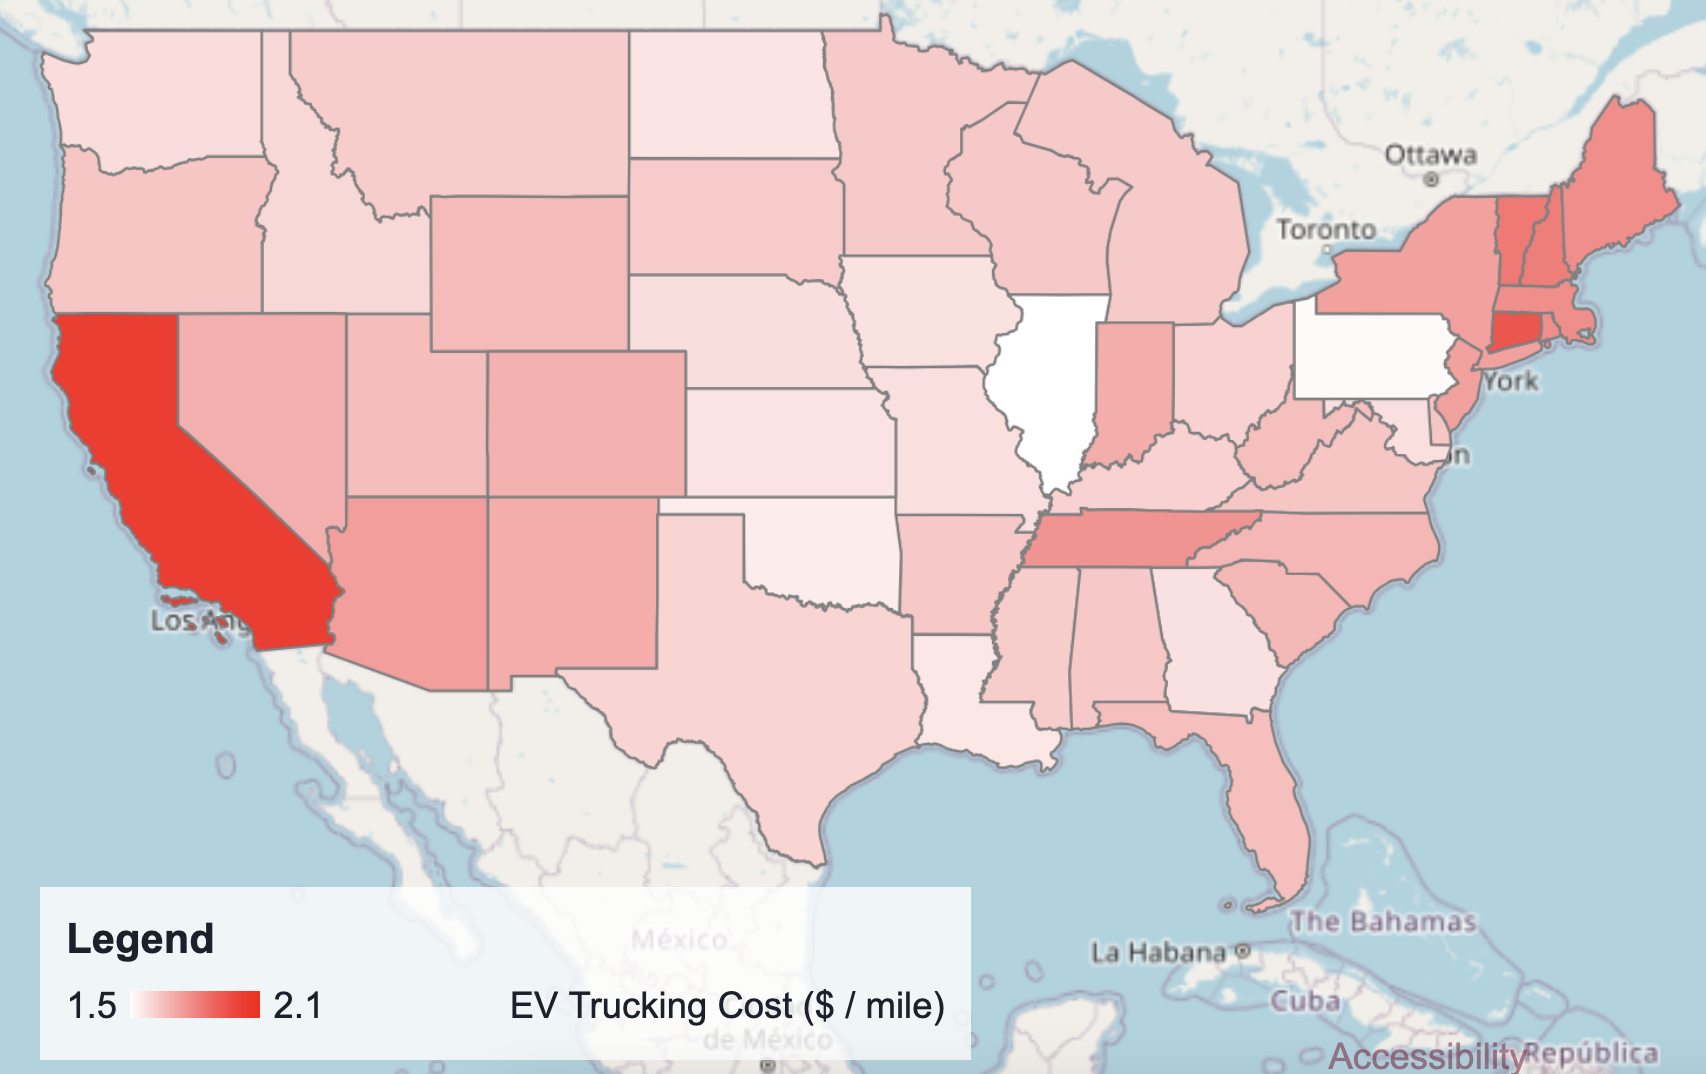
\includegraphics[width=\textwidth]{figures/ev_tco_map.png}
        \caption{Total cost of EV truck ownership}
        \label{fig:ev_tco_map}
    \end{subfigure}
    \hfill
    \begin{subfigure}[b]{0.49\textwidth}
        \centering
        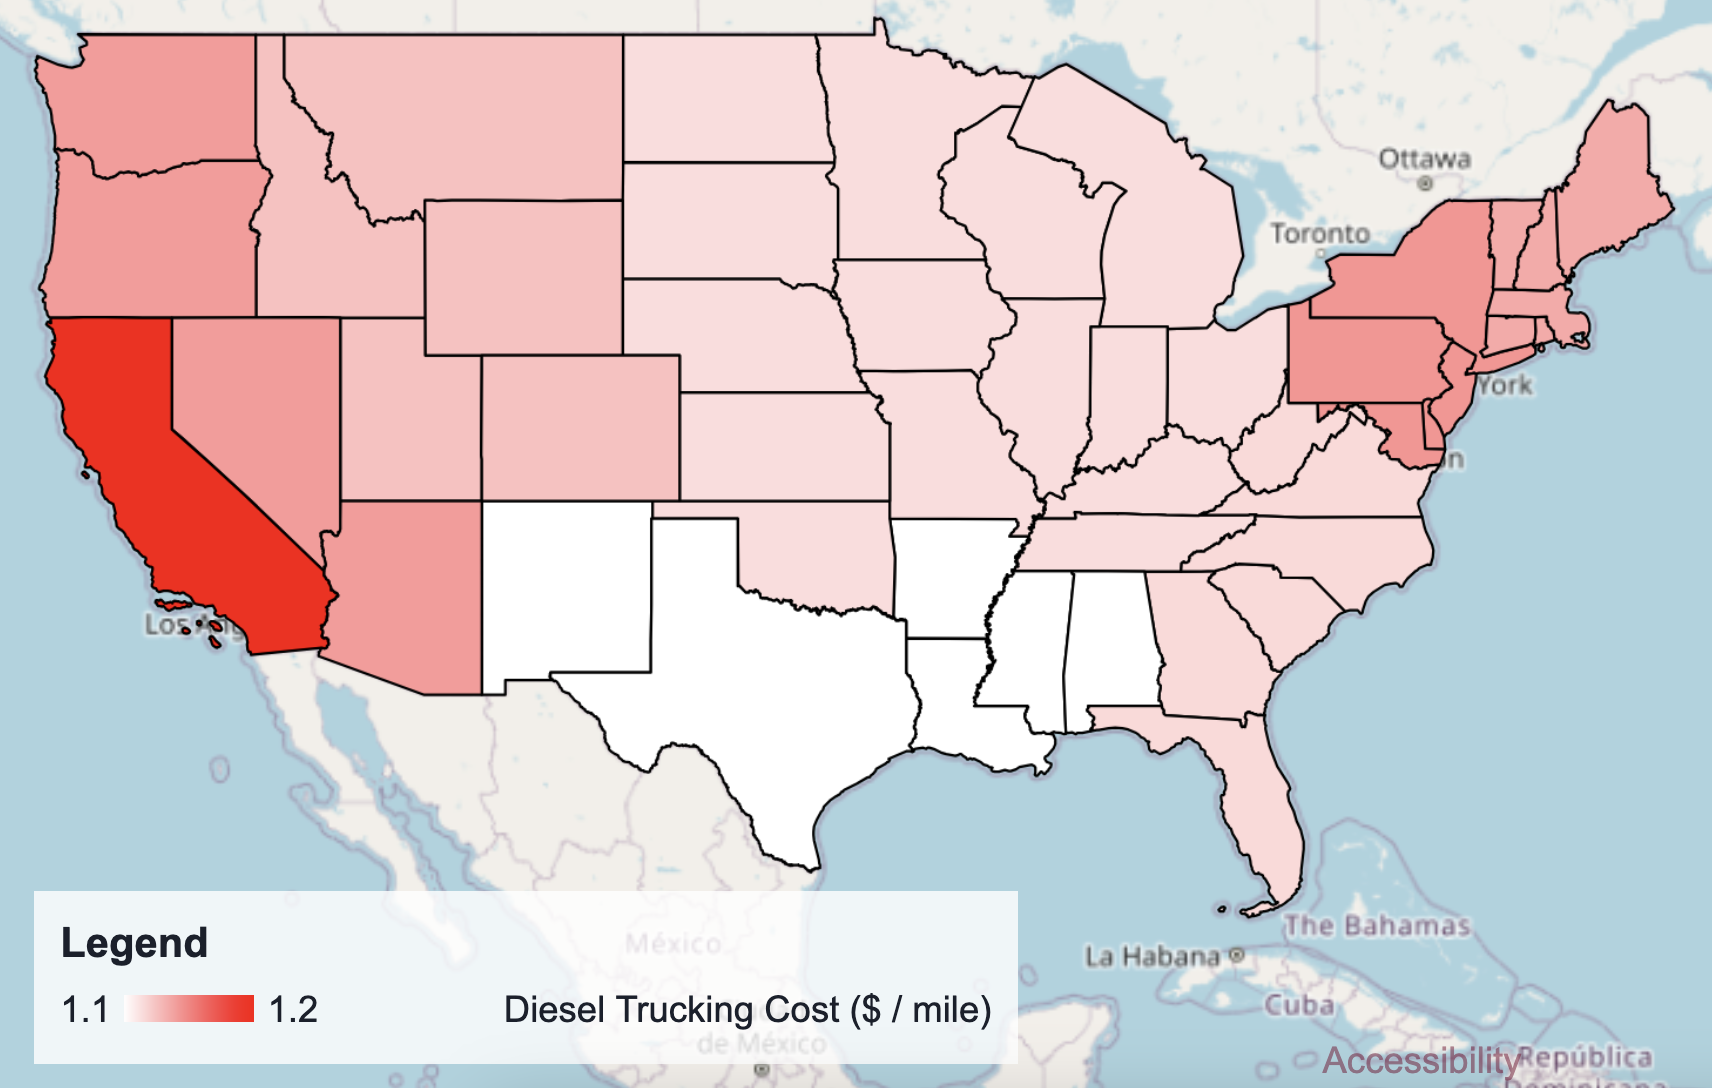
\includegraphics[width=\textwidth]{figures/diesel_tco_map.png}
        \caption{Total cost of diesel truck ownership}
        \label{fig:diesel_tco_map}
    \end{subfigure}
    \begin{subfigure}[b]{0.49\textwidth}
        \centering
        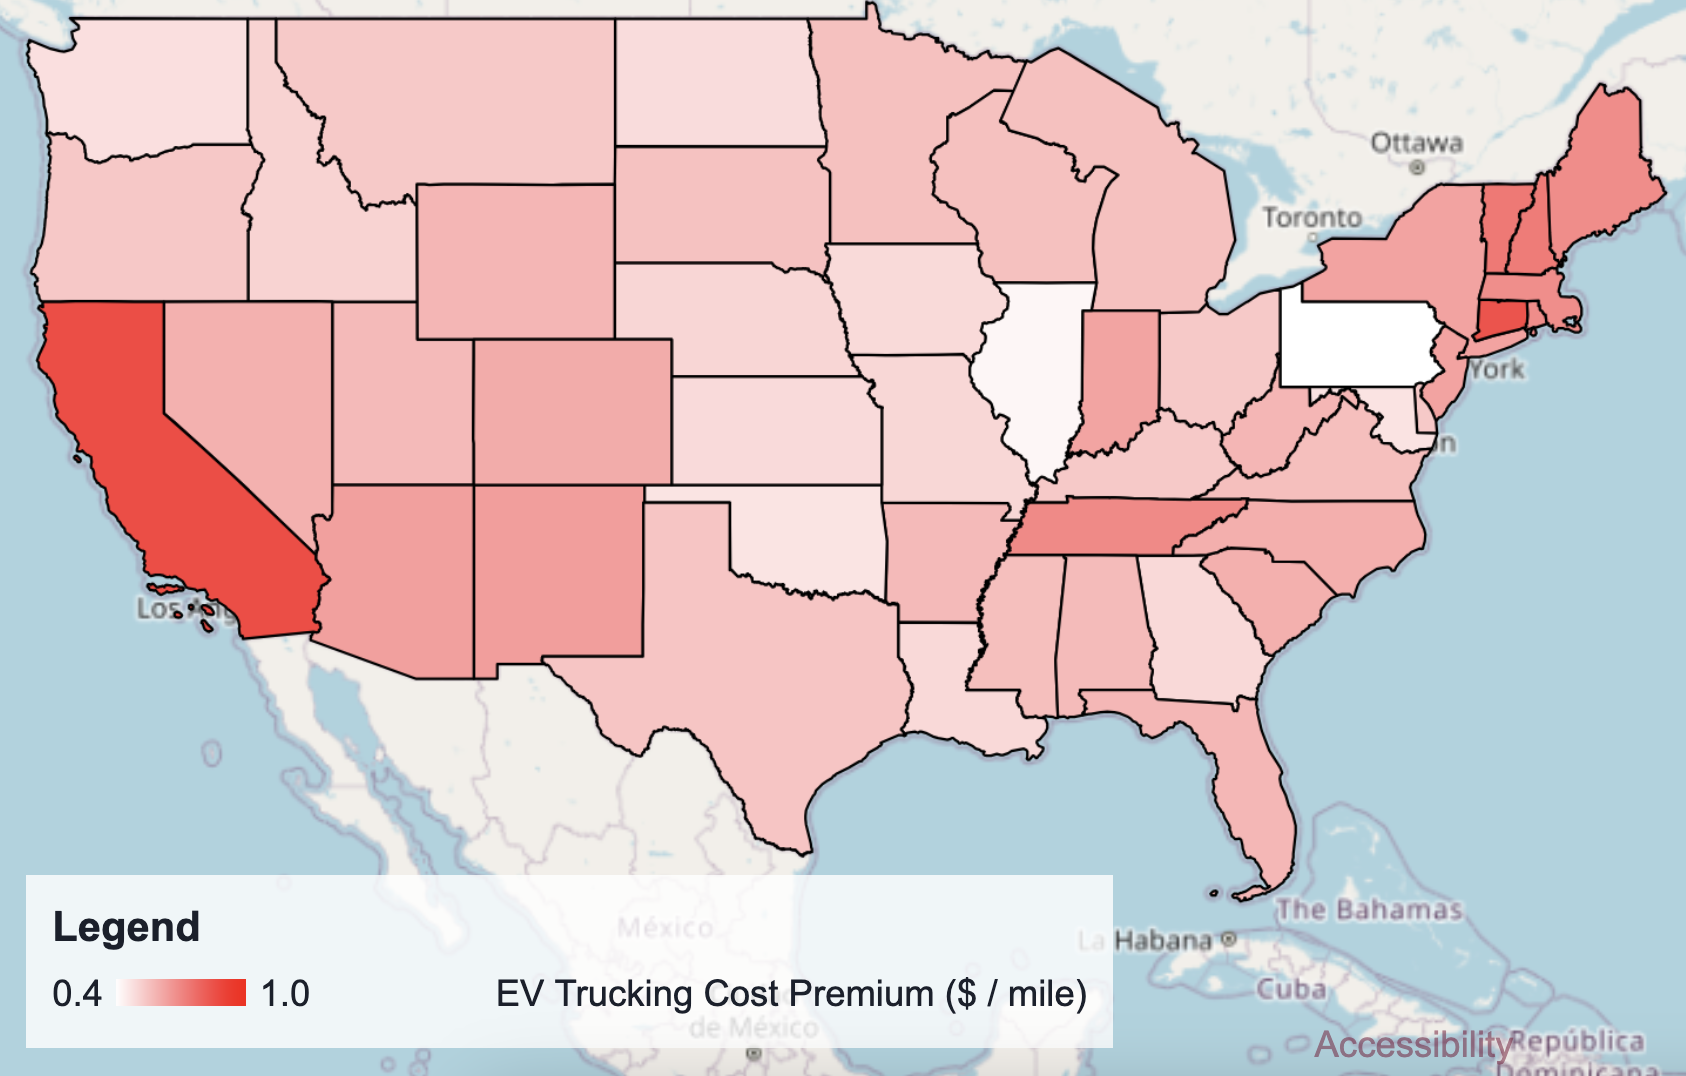
\includegraphics[width=\textwidth]{figures/ev_cost_premium_abs.png}
        \caption{TCO premium for EV trucking (absolute)}
        \label{fig:ev_cost_premium_abs}
    \end{subfigure}
    \hfill
    \begin{subfigure}[b]{0.49\textwidth}
        \centering
        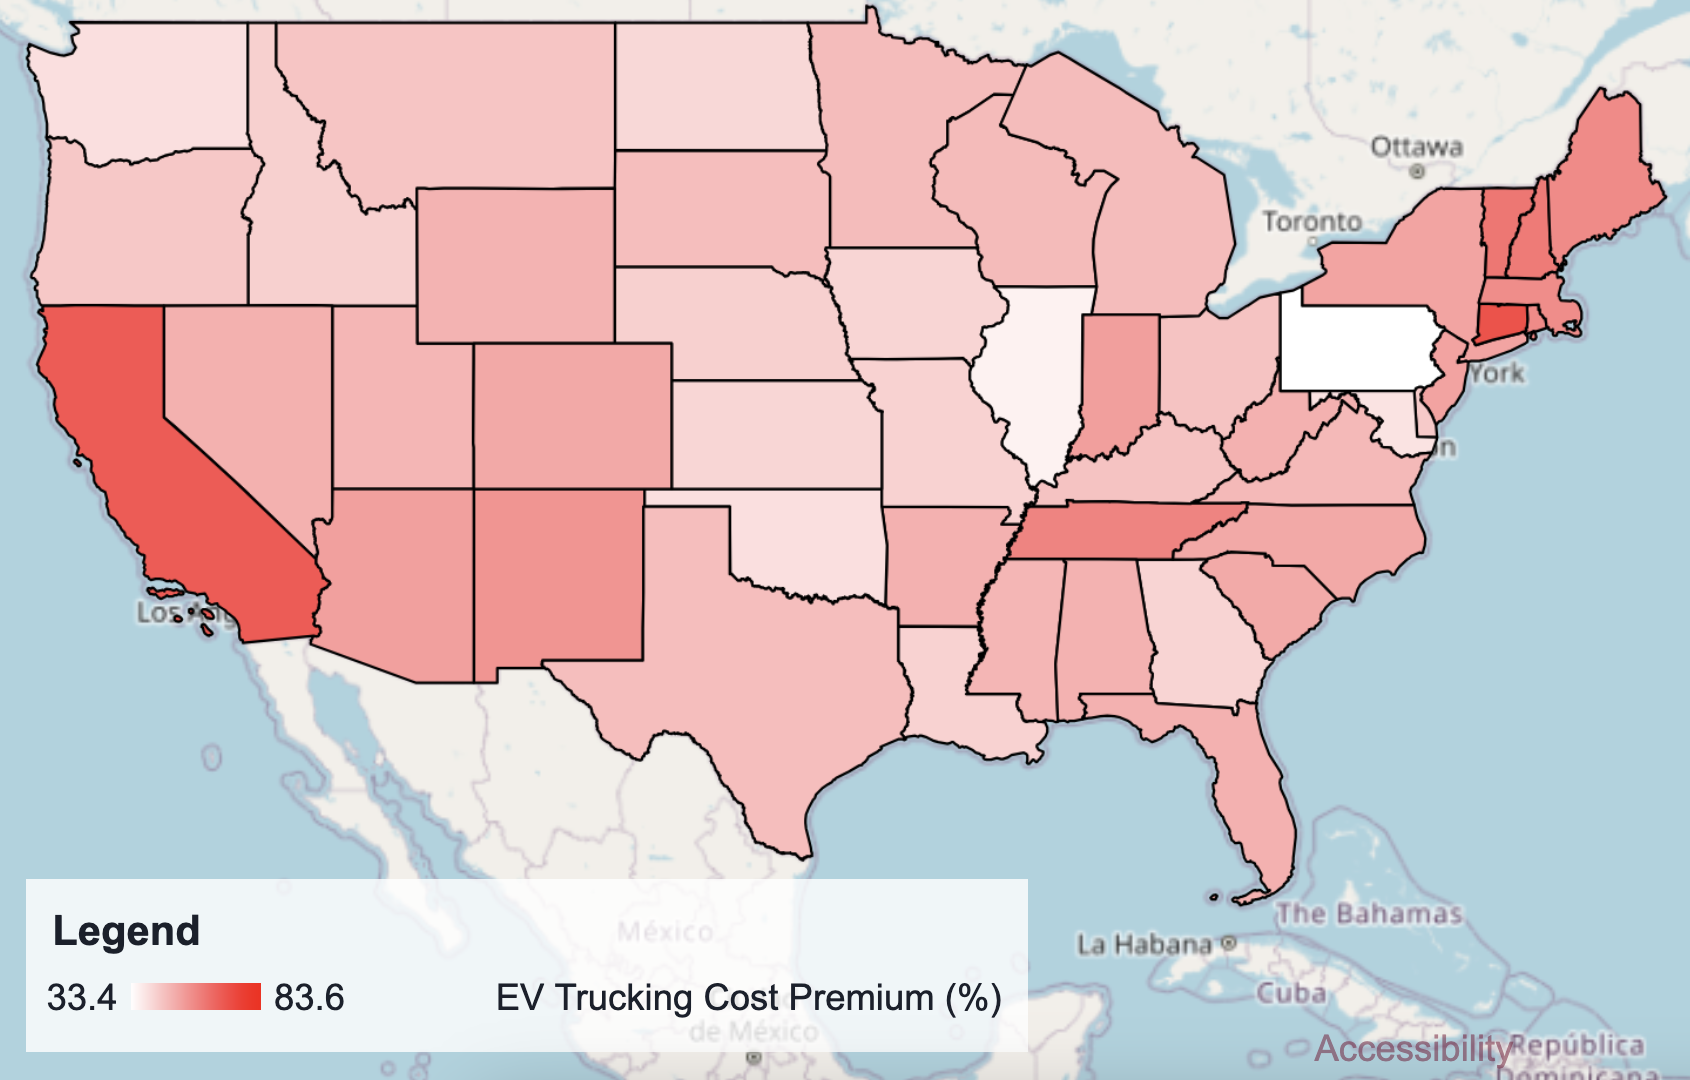
\includegraphics[width=\textwidth]{figures/ev_cost_premium_rel.png}
        \caption{TCO premium for EV trucking (relative)}
        \label{fig:ev_cost_premium_rel}
    \end{subfigure}
    \caption{Visualizations of the evaluated total cost of ownership (TCO) of EV and diesel trucks on the Geo-FTADS tool.}
    \label{fig:tco_maps}
\end{figure}